% ============================================================
%  BÁO CÁO PROJECT II - MỌNG FRUITBOXZ
%  Đại học Bách Khoa Hà Nội
% ============================================================
\documentclass[12pt, a4paper, oneside]{report}

% ---- Packages ----
\usepackage[utf8]{inputenc}
\usepackage[T1]{fontenc}
\usepackage[vietnamese]{babel}
\usepackage{fontspec}          % requires XeLaTeX or LuaLaTeX
\usepackage{geometry}
\usepackage{graphicx}
\usepackage{xcolor}
\usepackage{fancyhdr}
\usepackage{titlesec}
\usepackage{titletoc}
\usepackage{tocloft}
\usepackage{hyperref}
\usepackage{enumitem}
\usepackage{array}
\usepackage{booktabs}
\usepackage{longtable}
\usepackage{tabularx}
\usepackage{multirow}
\usepackage{caption}
\usepackage{subcaption}
\usepackage{float}
\usepackage{setspace}
\usepackage{microtype}
\usepackage{parskip}
\usepackage{etoolbox}
\usepackage{amsmath}
\usepackage{listings}
\usepackage{mdframed}
\usepackage{tikz}
\usepackage{pgf-umlsd}
\usetikzlibrary{arrows.meta, positioning, shapes.geometric, fit}

% ---- Page Layout ----
\geometry{
  top=25mm,
  bottom=25mm,
  left=30mm,
  right=20mm,
}

% ---- Font (XeLaTeX) ----
\setmainfont{Times New Roman}
\setsansfont{Arial}

% ---- Colors ----
\definecolor{primary}{RGB}{98, 0, 238}      % purple accent
\definecolor{secondary}{RGB}{0, 112, 192}   % blue accent
\definecolor{accentred}{RGB}{231, 76, 60}
\definecolor{lightgray}{RGB}{245, 245, 245}
\definecolor{darkgray}{RGB}{80, 80, 80}
\definecolor{tableheader}{RGB}{52, 73, 94}

% ---- Line Spacing ----
\setstretch{1.3}
\setlength{\emergencystretch}{2em}

% ---- Paragraph ----
\setlength{\parskip}{6pt}
\setlength{\parindent}{0pt}

% ---- Hyperref Setup ----
\hypersetup{
  colorlinks   = true,
  linkcolor    = secondary,
  citecolor    = secondary,
  urlcolor     = primary,
  pdftitle     = {Báo Cáo Project II - Mọng Fruitboxz},
  pdfauthor    = {Phan Anh Tài},
  pdfsubject   = {Website thương mại điện tử trái cây và hộp quà},
}

% ---- Chapter / Section Title Formatting ----
\titleformat{\chapter}[block]
  {\normalfont\Large\bfseries\color{secondary}}
  {Chương \thechapter:}{0.5em}{}
\titlespacing*{\chapter}{0pt}{20pt}{10pt}

\titleformat{\section}
  {\normalfont\large\bfseries\color{secondary}}
  {\thesection}{0.5em}{}
\titlespacing*{\section}{0pt}{12pt}{6pt}

\titleformat{\subsection}
  {\normalfont\normalsize\bfseries\color{darkgray}}
  {\thesubsection}{0.5em}{}
\titlespacing*{\subsection}{0pt}{10pt}{4pt}

\titleformat{\subsubsection}
  {\normalfont\normalsize\itshape\color{darkgray}}
  {\thesubsubsection}{0.5em}{}

% ---- Table of Contents ----
\renewcommand{\cftchapfont}{\bfseries}
\renewcommand{\cftsecfont}{}
\renewcommand{\cftsubsecfont}{}
\setlength{\cftbeforechapskip}{4pt}

% ---- Header / Footer ----
\pagestyle{fancy}
\setlength{\headheight}{14pt}
\fancyhf{}
\fancyhead[L]{\small\textit{Báo Cáo Project II}}
\fancyhead[R]{\small\textit{Phan Anh Tài - 20230063}}
\fancyfoot[C]{\thepage}
\renewcommand{\headrulewidth}{0.4pt}
\renewcommand{\footrulewidth}{0pt}

% Plain style for chapter first pages
\fancypagestyle{plain}{
  \fancyhf{}
  \fancyfoot[C]{\thepage}
  \renewcommand{\headrulewidth}{0pt}
}

% ---- Caption Formatting ----
\captionsetup{
  font=small,
  labelfont=bf,
  labelsep=period,
  justification=centering,
}

% ---- Figure Box ----
\newenvironment{figurebox}{%
  \begin{mdframed}[backgroundcolor=lightgray, linecolor=secondary!40,
    linewidth=0.8pt, innerleftmargin=6pt, innerrightmargin=6pt,
    innertopmargin=6pt, innerbottommargin=6pt]
}{%
  \end{mdframed}
}

% Diagram canvas. Keep pages in normal portrait orientation. Diagrams stay
% in the document flow and only move to the next page when there is not enough room.
\newenvironment{diagramcanvas}{%
  \par\medskip
}{%
  \par\medskip
}

% ---- Custom Commands ----
\newcommand{\keyword}[1]{\textbf{\textcolor{primary}{#1}}}
\newcommand{\role}[1]{\textit{\textcolor{secondary}{#1}}}
\newcommand{\techterm}[1]{\texttt{#1}}

% ============================================================
\begin{document}

% ---- Cover Page ----
% ============================================================
%  00_cover.tex  –  Trang bìa
% ============================================================
\begin{titlepage}
  \centering
  \thispagestyle{empty}

  % ---- University header ----
  {\Large\bfseries ĐẠI HỌC BÁCH KHOA HÀ NỘI}\\[4pt]
  {\large\bfseries TRƯỜNG CÔNG NGHỆ THÔNG TIN \& TRUYỀN THÔNG}\\[6pt]
  \rule{0.5\textwidth}{0.6pt}\\[20pt]

  % ---- University logo ----
  
\includegraphics[height=5cm]{images/logo-bach-khoa.png}\\[20pt]

  % ---- Report type ----
  {\LARGE\bfseries BÁO CÁO PROJECT II}\\[10pt]
  {\Large\bfseries ĐỀ TÀI:}\\[6pt]
  {\large\bfseries XÂY DỰNG WEBSITE THƯƠNG MẠI ĐIỆN TỬ}\\[4pt]
  {\Large\bfseries MỌNG FRUITBOXZ}\\[24pt]

  % ---- Info table ----
  \begin{tabular}{ll}
    \textbf{Học phần}              & : Project II \\[4pt]
    \textbf{Mã lớp}               & : 761982 \\[4pt]
    \textbf{Người thực hiện}       & : Phan Anh Tài \\[4pt]
    \textbf{Mã số sinh viên}       & : 20230063 \\[4pt]
    \textbf{Giảng viên hướng dẫn} & : Nguyễn Tấn Hùng \\
  \end{tabular}

  \vfill
  {\large\bfseries HÀ NỘI, 6/2026}
\end{titlepage}
\newpage


% ---- Front Matter ----
\pagenumbering{roman}
% ============================================================
%  00_loinoidau.tex – Lời nói đầu
% ============================================================
\chapter*{Lời Nói Đầu}
\addcontentsline{toc}{chapter}{Lời Nói Đầu}
\markboth{Lời Nói Đầu}{}

Thương mại điện tử đang trở thành một kênh bán hàng quan trọng đối với các cửa hàng thực phẩm tươi. Tuy nhiên, đặc thù của trái cây và hộp quà khiến bài toán không chỉ dừng ở việc hiển thị sản phẩm và nhận đơn. Hệ thống còn phải xử lý biến thể, giá bán, khuyến mãi, tồn kho nguyên liệu, giao hàng theo khu vực, nội dung truyền thông và trải nghiệm tư vấn trước khi mua.

Từ nhu cầu đó, đề tài \textit{``Xây dựng website thương mại điện tử Mọng Fruitboxz''} được thực hiện nhằm xây dựng một nền tảng bán trái cây tươi, sản phẩm cắt sẵn và hộp quà. Sản phẩm gồm ba phần chính: giao diện mua sắm dành cho khách hàng, giao diện quản trị dành cho nhân viên cửa hàng và hệ thống dịch vụ backend. Ngoài quy trình duyệt sản phẩm, giỏ hàng và đặt hàng, dự án còn triển khai tìm kiếm toàn văn, blog, quản lý nội dung, phân quyền, chatbot tư vấn và quản lý định mức nguyên liệu.

Về kỹ thuật, hệ thống sử dụng \techterm{React}, \techterm{Vite} và \techterm{Tailwind CSS} cho giao diện; \techterm{Medusa.js v2} và \techterm{Node.js} cho backend; \techterm{PostgreSQL}, \techterm{Redis}, \techterm{Meilisearch} và \techterm{MinIO} cho hạ tầng dữ liệu. Cách tiếp cận headless commerce giúp tách giao diện khỏi lõi nghiệp vụ, đồng thời tận dụng các mô-đun thương mại điện tử có sẵn của Medusa và mở rộng bằng các mô-đun riêng của cửa hàng.

Báo cáo này được viết lại trên cơ sở rà soát trực tiếp mã nguồn tại thời điểm tháng 6 năm 2026. Vì vậy, nội dung tập trung mô tả đúng những thành phần đã được triển khai, đồng thời chỉ rõ các giới hạn còn tồn tại và hướng hoàn thiện tiếp theo.

Tác giả xin chân thành cảm ơn giảng viên hướng dẫn, thầy \textbf{Nguyễn Tấn Hùng}, đã hỗ trợ và tạo điều kiện trong quá trình thực hiện đề tài.

\vspace{20pt}
\begin{flushright}
  \textit{Trân trọng,}\\[6pt]
  \textbf{Phan Anh Tài}
\end{flushright}
\newpage


\tableofcontents
\newpage

% ---- Main Chapters ----
\pagenumbering{arabic}
\setcounter{page}{1}

% ============================================================
%  01_gioithieu.tex – Chương 1: Giới thiệu bài toán
% ============================================================
\chapter{Giới Thiệu Bài Toán}

\section{Bối Cảnh}

Mọng Fruitboxz là mô hình cửa hàng kinh doanh trái cây tươi, trái cây cắt sẵn và hộp quà. Với mô hình này, khách hàng cần xem được sản phẩm theo nhu cầu, lựa chọn biến thể, biết rõ giá và phí giao hàng trước khi đặt mua. Ở phía cửa hàng, nhân viên cần một công cụ thống nhất để quản lý sản phẩm, đơn hàng, khách hàng, tồn kho, nội dung truyền thông và các chương trình khuyến mãi.

Nếu các nghiệp vụ trên được xử lý bằng nhiều công cụ rời rạc, dữ liệu giá, tồn kho và đơn hàng dễ mất đồng bộ. Việc tìm kiếm sản phẩm, theo dõi hiệu quả kinh doanh hoặc kiểm soát quyền thao tác của nhân viên cũng trở nên khó khăn. Do đó, đề tài hướng tới một nền tảng web tập trung nhưng vẫn có kiến trúc mô-đun để có thể mở rộng theo quy mô kinh doanh.

\section{Mục Tiêu Đề Tài}

Mục tiêu tổng quát là xây dựng một website thương mại điện tử có thể phục vụ trọn vẹn hành trình từ khám phá sản phẩm đến ghi nhận đơn hàng, đồng thời cung cấp công cụ vận hành cho cửa hàng. Các mục tiêu cụ thể gồm:

\begin{itemize}[leftmargin=2em, itemsep=3pt]
  \item Xây dựng catalog sản phẩm, danh mục, trang chi tiết, tìm kiếm và lọc sản phẩm.
  \item Hỗ trợ giỏ hàng, mã khuyến mãi, tính phí giao hàng và đặt hàng cho cả khách vãng lai lẫn khách đã đăng nhập.
  \item Cung cấp tài khoản khách hàng và khả năng tra cứu lịch sử đơn hàng.
  \item Xây dựng khu vực quản trị cho sản phẩm, danh mục, đơn hàng, khách hàng, khuyến mãi, tồn kho, nội dung và người dùng nội bộ.
  \item Quản lý tồn kho theo nguyên liệu và công thức cấu thành sản phẩm, phù hợp với sản phẩm trái cây cắt sẵn hoặc hộp phối sẵn.
  \item Tích hợp tìm kiếm toàn văn, lưu trữ ảnh, bộ nhớ đệm và chatbot tư vấn có cơ chế dự phòng.
  \item Tách biệt rõ giao diện, API, nghiệp vụ và hạ tầng để thuận tiện bảo trì, kiểm thử và triển khai.
\end{itemize}

\section{Phạm Vi Hệ Thống}

\subsection{Giao diện khách hàng}

Phần frontend cung cấp trang chủ, danh sách và chi tiết sản phẩm, danh mục, tìm kiếm, giỏ hàng, checkout, đăng ký/đăng nhập, tài khoản, lịch sử đơn, blog, liên hệ và các trang chính sách. Hệ thống còn có chức năng \textit{Hộp tự chọn}, cho phép khách xây dựng hộp trái cây theo nhu cầu.

\subsection{Giao diện quản trị}

Khu vực quản trị là một ứng dụng React trong cùng frontend, được bảo vệ bằng JWT và quyền RBAC. Nhân viên có thể truy cập dashboard, báo cáo tài chính, sản phẩm, danh mục, khách hàng, đơn hàng, khuyến mãi, kho, nguyên liệu, banner, blog, media, chatbot, cấu hình giao hàng và nội dung chính sách tùy theo quyền được cấp.

\subsection{Backend và hạ tầng}

Backend Medusa v2 cung cấp các mô-đun thương mại điện tử lõi và các API tùy biến. PostgreSQL lưu dữ liệu giao dịch; Redis hỗ trợ cache, event bus, rate limit và giỏ hàng phiên; Meilisearch lập chỉ mục tìm kiếm; MinIO lưu ảnh và tệp media. Các dịch vụ hạ tầng được mô tả bằng Docker Compose để thuận tiện khởi tạo môi trường phát triển.

\section{Đối Tượng Sử Dụng}

\begin{longtable}{@{}p{0.22\textwidth} p{0.70\textwidth}@{}}
  \toprule
  \textbf{Tác nhân} & \textbf{Quyền và nhu cầu chính} \\
  \midrule
  \endhead
  Khách vãng lai & Duyệt và tìm kiếm sản phẩm, quản lý giỏ hàng, nhận báo giá giao hàng, đặt đơn khách, đọc blog và hỏi chatbot. \\[3pt]
  Khách hàng & Có thêm khả năng quản lý tài khoản và xem lịch sử đơn hàng. \\[3pt]
  Nhân viên quản trị & Vận hành từng nhóm chức năng được cấp quyền, ví dụ sản phẩm, đơn hàng, khách hàng, nội dung hoặc kho. \\[3pt]
  Quản trị viên cấp cao & Quản lý người dùng nội bộ, vai trò, quyền hạn và toàn bộ cấu hình hệ thống. \\[3pt]
  Dịch vụ ngoài & Meilisearch phục vụ tìm kiếm; MinIO lưu media; Nominatim hỗ trợ địa chỉ; Groq cung cấp mô hình ngôn ngữ cho chatbot. \\
  \bottomrule
\end{longtable}

\section{Các Nhóm Chức Năng Chính}

\begin{enumerate}[leftmargin=2.2em, itemsep=4pt]
  \item \textbf{Catalog và nội dung:} sản phẩm, biến thể, danh mục, banner, blog và trang chính sách.
  \item \textbf{Bán hàng:} giỏ hàng, khuyến mãi, phí giao hàng, checkout, mã đơn và lịch sử đơn.
  \item \textbf{Tương tác khách hàng:} đăng ký, đăng nhập, liên hệ và chatbot tư vấn.
  \item \textbf{Vận hành:} quản lý đơn, khách hàng, tồn kho, công thức nguyên liệu và dashboard tài chính.
  \item \textbf{Quản trị hệ thống:} người dùng nội bộ, vai trò, quyền, cấu hình website, media và trạng thái tìm kiếm.
\end{enumerate}

\section{Yêu Cầu Phi Chức Năng}

\begin{itemize}[leftmargin=2em, itemsep=4pt]
  \item \textbf{Bảo mật:} xác thực bằng JWT, phân quyền ở cả giao diện và API, cấu hình CORS, giới hạn tần suất chatbot và không tin cậy giá tiền gửi từ trình duyệt.
  \item \textbf{Nhất quán dữ liệu:} backend truy vấn lại giá biến thể, kiểm tra định mức nguyên liệu và áp dụng khuyến mãi trước khi tạo đơn.
  \item \textbf{Khả dụng:} tìm kiếm và giỏ hàng có cơ chế dự phòng khi Meilisearch hoặc Redis chưa sẵn sàng.
  \item \textbf{Hiệu năng:} lazy loading các trang React, cache dữ liệu thường dùng và đồng bộ chỉ mục bằng subscriber theo sự kiện.
  \item \textbf{Khả năng mở rộng:} mô-đun tùy biến được tách khỏi lõi Medusa; hạ tầng lưu trữ, cache và tìm kiếm có thể triển khai độc lập.
  \item \textbf{Khả năng sử dụng:} giao diện responsive, hỗ trợ tiếng Việt và tiếng Anh, có trạng thái loading, empty, error và phản hồi thao tác.
\end{itemize}

\section{Kết Cấu Báo Cáo}

Chương 2 đặc tả yêu cầu và các luồng nghiệp vụ. Chương 3 trình bày kiến trúc, thành phần và luồng xử lý. Chương 4 mô tả mô hình dữ liệu. Chương 5 phân tích các nhóm giao diện. Chương 6 tổng kết kết quả, giới hạn và hướng phát triển.

% ============================================================
%  02_dacta.tex – Chương 2: Đặc tả yêu cầu
% ============================================================
\chapter{Đặc Tả Yêu Cầu}

\section{Mục Đích và Phạm Vi Đặc Tả}

Chương này mô tả các yêu cầu được rút ra từ mã nguồn hiện tại, thay vì mô tả một hệ thống giả định. Mỗi yêu cầu được gắn với tác nhân, đầu vào, kết quả và trạng thái triển khai. Cách tiếp cận này giúp báo cáo có thể dùng làm tài liệu kiểm tra chéo giữa giao diện, API và dữ liệu.

\section{Công Nghệ và Ràng Buộc}

\begin{longtable}{@{}p{0.22\textwidth} p{0.25\textwidth} p{0.45\textwidth}@{}}
  \toprule
  \textbf{Thành phần} & \textbf{Công nghệ} & \textbf{Vai trò trong dự án} \\
  \midrule
  \endhead
  Frontend & React 19, Vite 7, Tailwind CSS 4 & Giao diện mua sắm và khu vực quản trị tùy biến. \\[3pt]
  Backend & Medusa.js 2.15, Node.js 20, TypeScript & API, mô-đun thương mại điện tử, xác thực và nghiệp vụ. \\[3pt]
  Cơ sở dữ liệu & PostgreSQL 15 & Dữ liệu giao dịch, catalog, người dùng và mô-đun tùy biến. \\[3pt]
  Cache và sự kiện & Redis 7 & Cache, event bus, rate limit và đồng bộ giỏ hàng phiên khi được bật. \\[3pt]
  Tìm kiếm & Meilisearch 1.13 & Lập chỉ mục và tìm kiếm sản phẩm theo từ khóa, danh mục, mức giá. \\[3pt]
  Lưu trữ đối tượng & MinIO, giao thức S3 & Ảnh sản phẩm, banner và media quản trị. \\[3pt]
  AI tư vấn & Groq API & Sinh câu trả lời từ FAQ và ngữ cảnh sản phẩm, có fallback khi dịch vụ lỗi. \\[3pt]
  Môi trường & Docker Compose & Khởi tạo PostgreSQL, Redis, Meilisearch và MinIO cục bộ. \\
  \bottomrule
\end{longtable}

Backend yêu cầu Node.js phiên bản từ 20 đến dưới 23; cấu hình của dự án khuyến nghị Node 20 LTS. Frontend gọi API thông qua Medusa JS SDK; địa chỉ backend và publishable key được lấy từ biến môi trường.

\section{Danh Sách Use Case}

\begin{longtable}{@{}p{0.10\textwidth} p{0.25\textwidth} p{0.20\textwidth} p{0.37\textwidth}@{}}
  \toprule
  \textbf{Mã} & \textbf{Use case} & \textbf{Tác nhân} & \textbf{Kết quả mong đợi} \\
  \midrule
  \endhead
  UC01 & Duyệt catalog & Mọi khách & Xem danh sách, danh mục và chi tiết sản phẩm đang bán. \\
  UC02 & Tìm kiếm sản phẩm & Mọi khách & Nhận kết quả theo từ khóa, bộ lọc và thứ tự; fallback khi máy tìm kiếm lỗi. \\
  UC03 & Quản lý giỏ hàng & Mọi khách & Thêm, xóa, đổi số lượng; lưu cục bộ và đồng bộ phiên khi có Redis. \\
  UC04 & Đăng ký/đăng nhập & Khách hàng & Nhận JWT hợp lệ và truy cập chức năng tài khoản. \\
  UC05 & Đặt hàng & Khách hoặc khách hàng & Backend xác minh giá, tồn kho, phí ship, mã giảm giá và tạo đơn. \\
  UC06 & Xem lịch sử đơn & Khách hàng & Chỉ xem các đơn gắn với định danh khách đang đăng nhập. \\
  UC07 & Hộp tự chọn & Mọi khách & Chọn thành phần hộp theo cấu hình sản phẩm và thêm vào giỏ. \\
  UC08 & Tư vấn chatbot & Mọi khách & Trả lời dựa trên FAQ và kết quả catalog; ghi log câu hỏi chưa giải quyết. \\
  UC09 & Quản lý catalog & Nhân viên có quyền & Tạo/sửa sản phẩm, danh mục, công thức và dữ liệu tồn kho. \\
  UC10 & Quản lý đơn hàng & Nhân viên có quyền & Tra cứu chi tiết và cập nhật trạng thái xử lý đơn. \\
  UC11 & Quản lý nội dung & Nhân viên có quyền & Quản lý banner, blog, media, FAQ và các trang chính sách. \\
  UC12 & Báo cáo vận hành & Nhân viên có quyền & Xem chỉ số doanh thu, chi phí, lợi nhuận và dữ liệu tổng hợp. \\
  UC13 & Quản lý người dùng và RBAC & Quản trị viên & Gán vai trò, quyền và giới hạn chức năng theo mô-đun/hành động. \\
  \bottomrule
\end{longtable}

Hình~\ref{fig:use-case-overview} nhóm các use case theo hai tác nhân chính. Đây là sơ đồ tổng quan; các điều kiện và luồng thay thế được đặc tả chi tiết ở các mục tiếp theo.

\begin{diagramcanvas}
\begin{figure}[H]
  \centering
  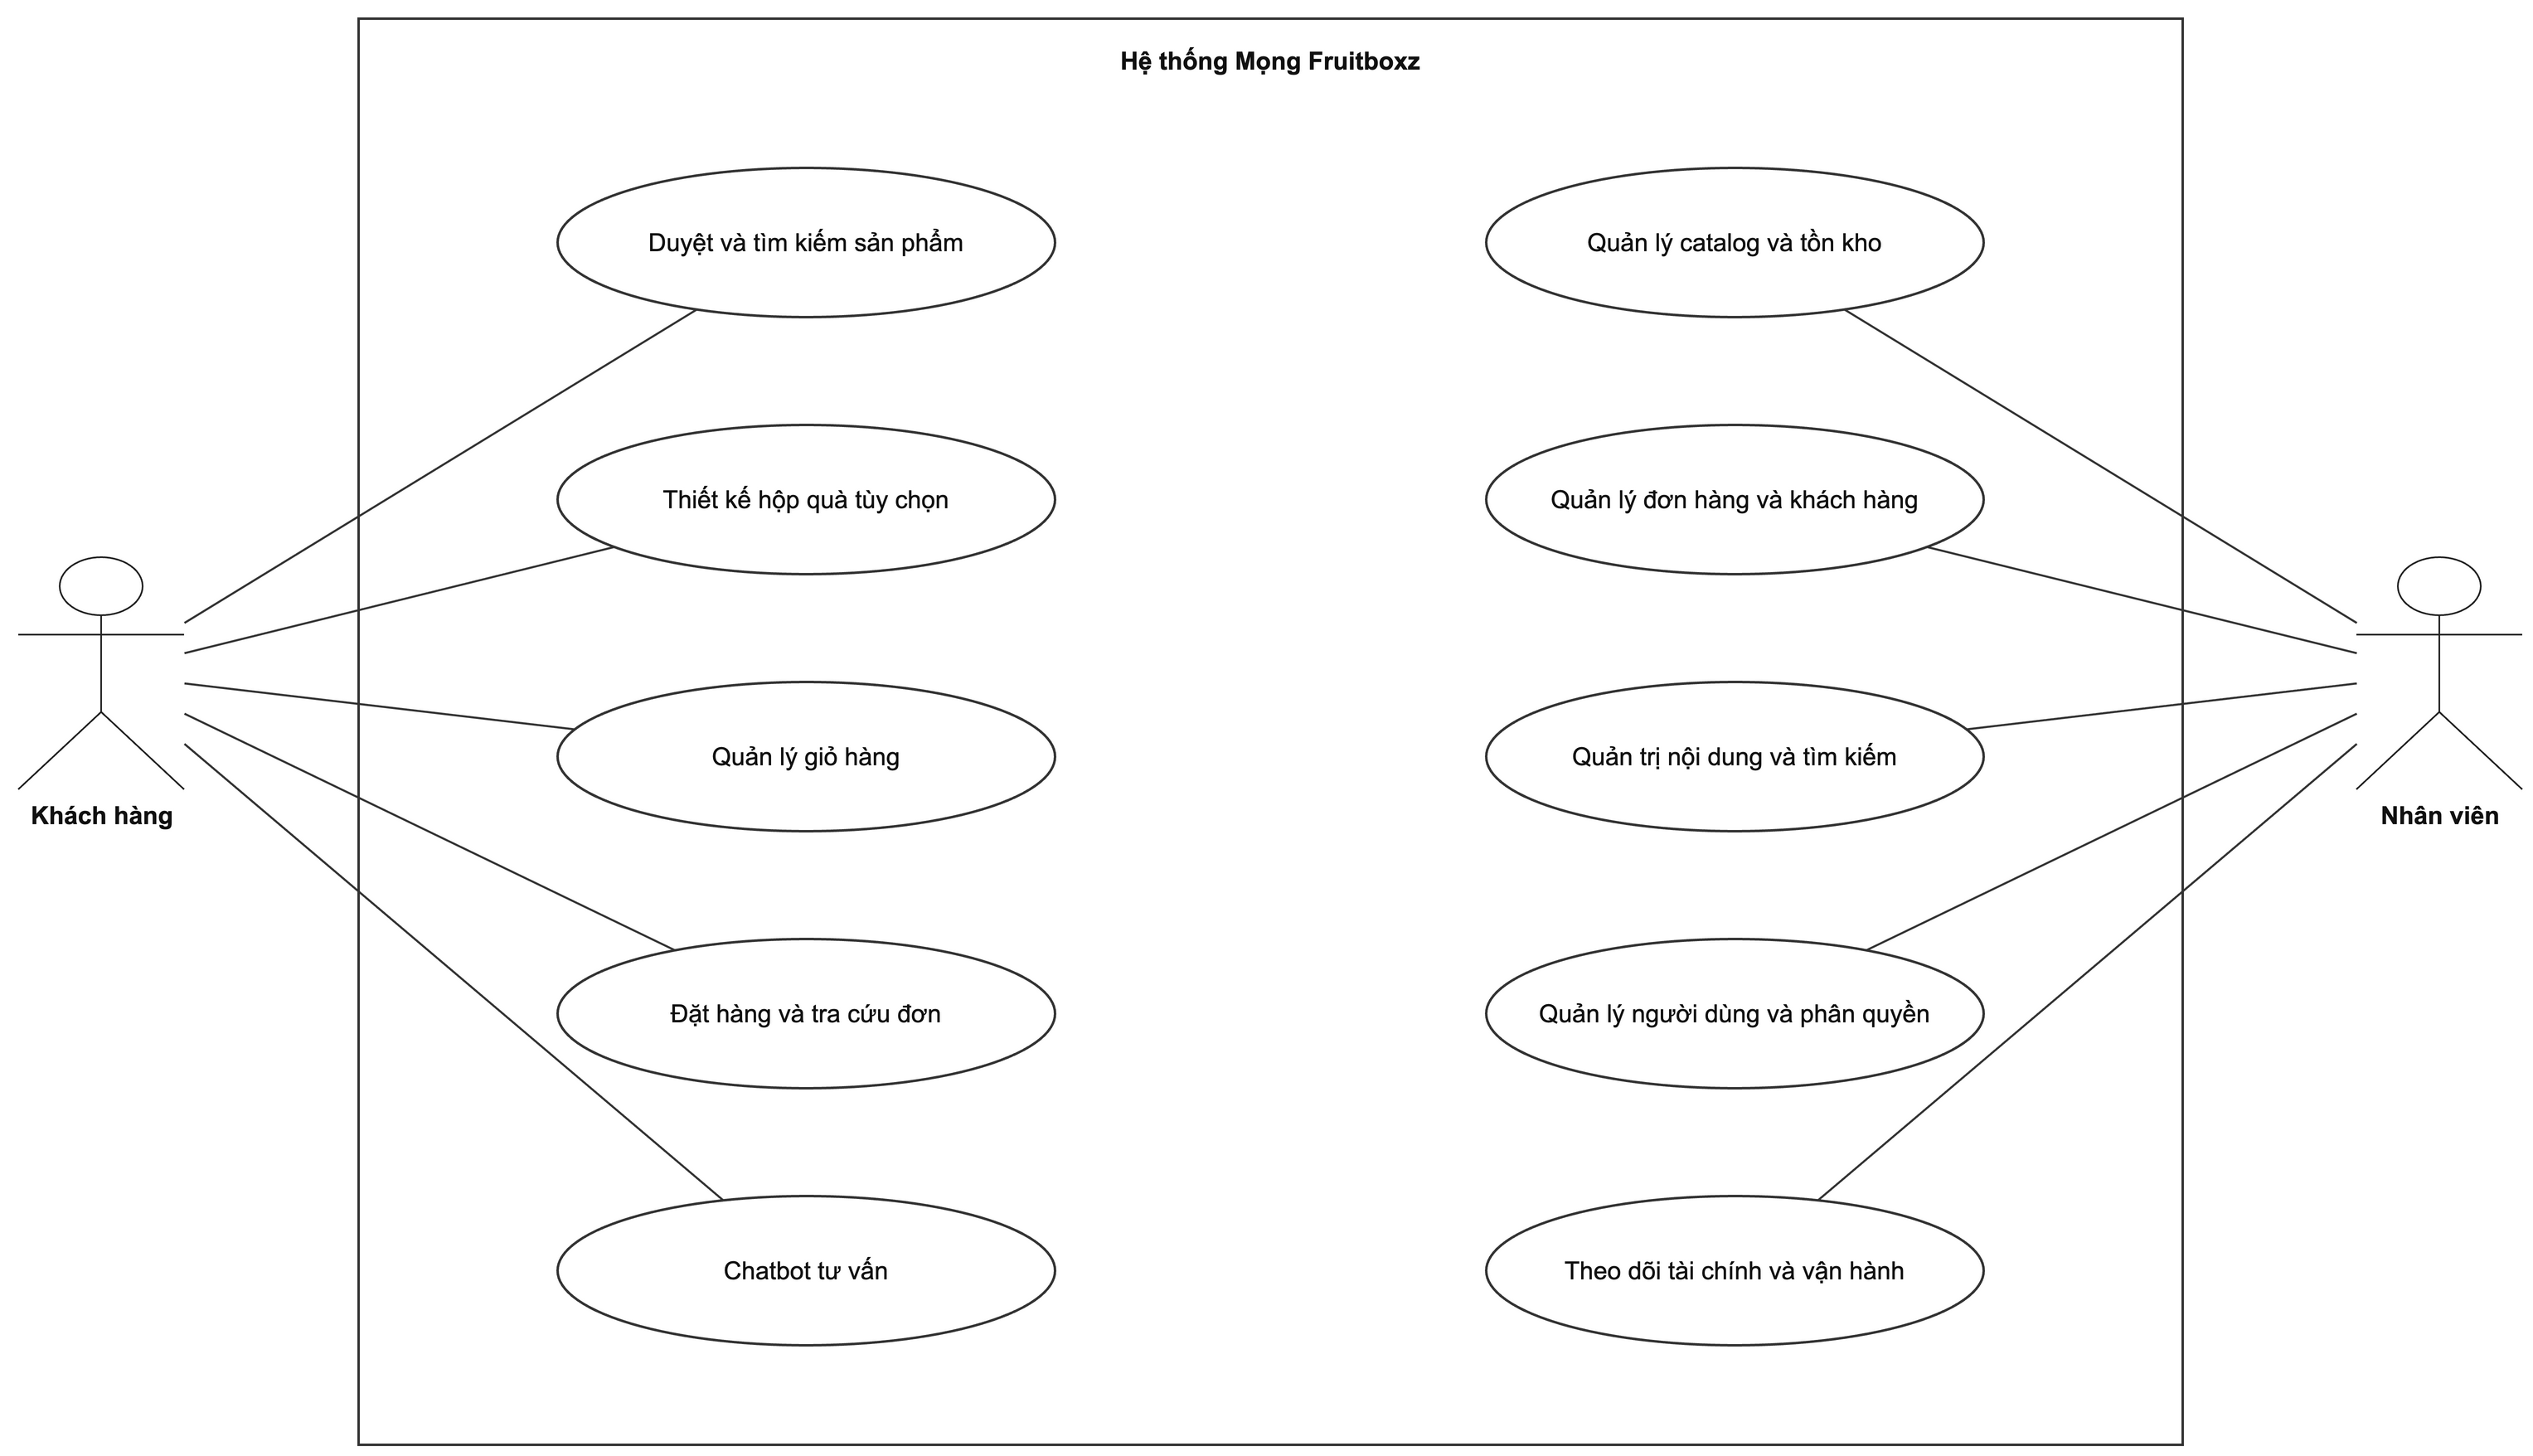
\includegraphics[width=\linewidth,height=0.48\textheight,keepaspectratio]{images/use-case.drawio.png}
  \caption{Use case tổng quan của hệ thống Mọng Fruitboxz}
  \label{fig:use-case-overview}
\end{figure}
\end{diagramcanvas}

\subsection{Quy ước mô hình hóa}

Các sơ đồ trong báo cáo tuân theo quy ước UML được sử dụng trong học phần: tác nhân nằm ngoài biên hệ thống; use case được biểu diễn bằng hình ellipse; quan hệ \textit{include}/\textit{extend} dùng đường nét đứt và mũi tên phụ thuộc; lớp có các ngăn tên--thuộc tính; biểu đồ trình tự đọc từ trên xuống; trạng thái chỉ nối bằng các chuyển tiếp có ý nghĩa nghiệp vụ. Màu sắc chỉ dùng để phân vùng hoặc làm tiêu đề, không mã hóa thêm ngữ nghĩa khi chưa có chú giải. Cách trình bày này giúp người đọc phân biệt rõ sơ đồ phân tích với ảnh giao diện và sơ đồ triển khai.

\section{Đặc Tả Các Luồng Nghiệp Vụ Chính}

\subsection{UC02 -- Tìm kiếm sản phẩm}

\begin{longtable}{@{}p{0.23\textwidth}p{0.69\textwidth}@{}}
  \toprule
  \textbf{Thuộc tính} & \textbf{Đặc tả} \\
  \midrule
  Tác nhân & Mọi khách truy cập. \\
  Tiền điều kiện & Frontend kết nối được backend; Meilisearch là thành phần tối ưu tùy chọn. \\
  Kích hoạt & Người dùng nhập từ khóa hoặc đổi danh mục, mức giá, thứ tự sắp xếp. \\
  Luồng chính & (1) Gửi tiêu chí tìm kiếm; (2) chỉ lấy product \texttt{published}; (3) áp dụng filter, sort và phân trang; (4) trả tên, slug, ảnh, giá, danh mục và trạng thái tồn. \\
  Luồng thay thế & Nếu Meilisearch lỗi hoặc chưa cấu hình, backend dùng Medusa Query, chuẩn hóa chuỗi và lọc catalog tại ứng dụng. \\
  Hậu điều kiện & Danh sách kết quả và tổng số bản ghi khớp tiêu chí được hiển thị; dữ liệu không bị thay đổi. \\
  \bottomrule
\end{longtable}

\subsection{UC03 -- Quản lý giỏ hàng}

\begin{longtable}{@{}p{0.23\textwidth}p{0.69\textwidth}@{}}
  \toprule
  \textbf{Thuộc tính} & \textbf{Đặc tả} \\
  \midrule
  Tác nhân & Mọi khách truy cập. \\
  Tiền điều kiện & Sản phẩm có biến thể hợp lệ và còn khả năng mua. \\
  Luồng chính & Thêm sản phẩm, đổi số lượng, chọn dòng hàng hoặc xóa; reducer cập nhật trạng thái và lưu \techterm{localStorage}. \\
  Đồng bộ & Mỗi trình duyệt có session ID; frontend thử đồng bộ qua \texttt{/store/session-cart/:id} khi Redis hoạt động. \\
  Luồng suy giảm & Redis lỗi không chặn mua hàng; localStorage trở thành nguồn dữ liệu hoạt động. Ảnh cũ được đối chiếu lại thumbnail từ catalog. \\
  Hậu điều kiện & Tổng số lượng và tạm tính được cập nhật; giỏ còn tồn tại sau khi tải lại trang. \\
  \bottomrule
\end{longtable}

\subsection{UC05 -- Đặt hàng}

\begin{longtable}{@{}p{0.23\textwidth}p{0.69\textwidth}@{}}
  \toprule
  \textbf{Thuộc tính} & \textbf{Đặc tả} \\
  \midrule
  Tác nhân & Khách vãng lai hoặc khách hàng đã đăng nhập. \\
  Tiền điều kiện & Giỏ có ít nhất một dòng hàng; tên, điện thoại và địa chỉ hợp lệ. Email là tùy chọn. \\
  Đầu vào & \texttt{variant\_id}, số lượng, thông tin người nhận, địa chỉ hoặc tọa độ, mã khuyến mãi; backend hỗ trợ khóa idempotency tùy chọn. \\
  Luồng chuẩn bị & Người dùng có thể cho phép định vị. Frontend gọi reverse geocode để điền địa chỉ; mỗi khi địa chỉ/tọa độ thay đổi, hiệu ứng debounce 300 ms tự gọi \texttt{/store/shipping/quote} và cập nhật phí, chế độ tính cùng khoảng cách ước lượng. \\
  Luồng chính & (1) Xác thực payload; (2) nếu có khóa idempotency thì tìm đơn đã xử lý; (3) tải lại biến thể và giá VND; (4) tính nhu cầu BOM, kiểm tra tồn; (5) tính lại ship và promotion tại server; (6) tạo order \texttt{pending} và mã \texttt{MONG-...}; (7) phát \texttt{order.placed}; (8) trả order và bảng tổng hợp. \\
  Luồng lỗi & Từ chối khi biến thể không tồn tại, thiếu giá, thiếu nguyên liệu, promotion không hợp lệ hoặc dữ liệu giao hàng sai. Nếu reverse geocode lỗi, giữ tọa độ và yêu cầu người dùng bổ sung địa chỉ; nếu API quote lỗi, frontend dùng ước lượng cục bộ. \\
  Quy tắc tin cậy & Không dùng giá/tổng tiền gửi từ trình duyệt làm nguồn chuẩn. Phí giao hàng và giảm giá được tính lại ở backend; idempotency chỉ có hiệu lực khi client cung cấp khóa. \\
  Hậu điều kiện & Order và metadata giao hàng được lưu; frontend xóa giỏ và hiển thị mã đơn, tổng thanh toán cùng QR chuyển khoản. \\
  \bottomrule
\end{longtable}

Hình~\ref{fig:checkout-activity} mô tả luồng nghiệp vụ từ góc nhìn trách nhiệm; Hình~\ref{fig:shipping-quote-sequence} mô tả bước định vị và báo phí; Hình~\ref{fig:checkout-flow} mô tả các bước kiểm tra khi tạo đơn. Như vậy UC05 được đặc tả bằng cả bảng văn bản, biểu đồ hoạt động và các sơ đồ luồng, phù hợp cách mô hình hóa chức năng--hành vi trong slide học phần.

\subsubsection{Bảng quyết định phí giao hàng}

\begin{longtable}{@{}p{0.29\textwidth}p{0.25\textwidth}p{0.38\textwidth}@{}}
  \toprule
  \textbf{Điều kiện} & \textbf{Chế độ} & \textbf{Kết quả} \\
  \midrule
  Chưa có địa chỉ/tọa độ & \texttt{fallback-empty} & Dùng phí Hà Nội mặc định để tạm tính. \\
  Ngoài Hà Nội & \texttt{static-non-hanoi} & Dùng mức phí ngoài Hà Nội từ cấu hình. \\
  Quận thuộc danh sách miễn phí & \texttt{district-free} & Phí giao hàng bằng 0. \\
  Khớp quận hoặc có tọa độ & \texttt{distance-estimate} & Khoảng cách đường đi ước lượng bằng Haversine $\times 1{,}3$; phí = phí nền + đơn giá/km, làm tròn nghìn và chặn min--max. \\
  Có địa chỉ Hà Nội nhưng không khớp quận & \texttt{static-hanoi} & Dùng phí Hà Nội mặc định. \\
  API quote không khả dụng & \texttt{fallback} ở frontend & Ước lượng cục bộ theo quận đã nhận diện; nếu không nhận diện được thì dùng phí mặc định. \\
  \bottomrule
\end{longtable}

\subsection{UC08 -- Chatbot tư vấn}

\begin{longtable}{@{}p{0.23\textwidth}p{0.69\textwidth}@{}}
  \toprule
  \textbf{Thuộc tính} & \textbf{Đặc tả} \\
  \midrule
  Tác nhân & Mọi khách truy cập. \\
  Đầu vào & Câu hỏi tự nhiên; không nhận dữ liệu đơn hàng hoặc thông tin thanh toán. \\
  Luồng chính & Chuẩn hóa câu hỏi, tìm FAQ và tối đa bốn sản phẩm liên quan, tạo prompt có ngữ cảnh rồi gọi Groq. \\
  Ràng buộc & Không bịa sản phẩm, không tiết lộ prompt, không truy cập dữ liệu cá nhân; có rate limit theo IP và cache câu trả lời. \\
  Luồng thay thế & Trả FAQ trực tiếp; nếu AI lỗi thì dùng kết quả catalog hoặc hướng dẫn liên hệ hotline. \\
  Hậu điều kiện & Nội dung trả lời, chế độ phản hồi và trạng thái resolved được ghi vào chatbot log. \\
  \bottomrule
\end{longtable}

\subsection{UC13 -- Phân quyền quản trị}

\begin{longtable}{@{}p{0.23\textwidth}p{0.69\textwidth}@{}}
  \toprule
  \textbf{Thuộc tính} & \textbf{Đặc tả} \\
  \midrule
  Tác nhân & Người dùng quản trị đã được cấp tài khoản. \\
  Tiền điều kiện & JWT admin hợp lệ; metadata chứa danh sách role hiện hành. \\
  Luồng chính & Tải permission; giao diện dùng \texttt{RequirePermission}; backend ánh xạ route và HTTP method sang \texttt{module.action}, sau đó cho phép hoặc trả 403. \\
  Quy tắc & Kiểm tra quyền bắt buộc ở backend; ẩn menu chỉ là biện pháp UX. Super admin dùng permission đại diện \texttt{*}. \\
  Hậu điều kiện & Chỉ các route và thao tác được cấp quyền mới thực thi; thay đổi role phản ánh khi tải lại quyền. \\
  \bottomrule
\end{longtable}

\section{Truy Vết Yêu Cầu Sang Thiết Kế}

\begin{longtable}{@{}p{0.15\textwidth}p{0.27\textwidth}p{0.25\textwidth}p{0.25\textwidth}@{}}
  \toprule
  \textbf{Use case} & \textbf{Mô hình hành vi} & \textbf{Thành phần thực thi} & \textbf{Bằng chứng giao diện} \\
  \midrule
  UC02 & Use case tổng quan & Search API, Meilisearch, fallback Query & Hình~\ref{fig:ui-discovery} \\
  UC03 & Activity checkout, bước chuẩn bị giỏ & \texttt{CartContext}, session cart & Hình~\ref{fig:ui-assist-checkout} \\
  UC05 & Activity, luồng định vị/báo phí, luồng tạo đơn, state order & Checkout UI/API, geocode, quote, Ingredient, Order, Event Bus & Hình~\ref{fig:ui-assist-checkout} \\
  UC08 & Sequence chatbot & Chatbot API, FAQ/catalog retrieval, Groq & Hình~\ref{fig:ui-assist-checkout} \\
  UC09--UC13 & Module, class, ERD và deployment & Admin routes, RBAC, module service & Hình~\ref{fig:ui-admin-overview} và \ref{fig:ui-admin-operations} \\
  \bottomrule
\end{longtable}

\section{Yêu Cầu Phi Chức Năng}

\begin{longtable}{@{}p{0.22\textwidth} p{0.70\textwidth}@{}}
  \toprule
  \textbf{Thuộc tính} & \textbf{Yêu cầu và cách kiểm chứng} \\
  \midrule
  \endhead
  Hiệu năng & Route giao diện được tách bundle; ảnh tải lười; tìm kiếm ưu tiên chỉ mục Meilisearch và có phân trang. \\
  Tin cậy & Checkout dùng khóa idempotency; giá được xác minh tại server; cache, Redis và tìm kiếm đều có phương án suy giảm chức năng. \\
  Bảo mật & JWT tách customer/admin; backend kiểm tra RBAC; payload được xác thực; secret lấy từ biến môi trường. \\
  Khả dụng & Luồng browse--cart--checkout có thông báo loading/error; các trang chính hoạt động ở kích thước desktop và mobile. \\
  Bảo trì & API chia namespace, nghiệp vụ chia module, migration đi cùng module và thành phần giao diện được tái sử dụng. \\
  Quan sát & Lỗi API có mã trạng thái rõ; chatbot lưu log câu hỏi; production cần bổ sung structured log và metric. \\
  \bottomrule
\end{longtable}

\section{Yêu Cầu Dữ Liệu và Kiểm Tra Hợp Lệ}

\begin{itemize}[leftmargin=2em, itemsep=4pt]
  \item Định danh sản phẩm và biến thể phải tồn tại tại thời điểm checkout.
  \item Số lượng mua phải là số nguyên dương và không vượt quá lượng nguyên liệu khả dụng.
  \item Giá đơn hàng luôn được lấy từ backend và dùng tiền tệ VND.
  \item Email, số điện thoại, địa chỉ và payload contact/chatbot được kiểm tra qua middleware Zod.
  \item Khách vãng lai không được tự động gắn đơn vào tài khoản đã tồn tại chỉ dựa trên email.
  \item API admin yêu cầu xác thực; các mô-đun nhạy cảm yêu cầu thêm quyền RBAC tương ứng.
\end{itemize}

\section{Tiêu Chí Chấp Nhận}

\begin{longtable}{@{}p{0.28\textwidth} p{0.64\textwidth}@{}}
  \toprule
  \textbf{Nhóm} & \textbf{Tiêu chí} \\
  \midrule
  \endhead
  Catalog & Sản phẩm xuất bản hiển thị đúng tên, ảnh, giá, biến thể và danh mục. \\
  Checkout & Không tạo đơn nếu giá/tồn kho không hợp lệ; tổng tiền thể hiện được giảm giá và phí giao hàng. \\
  Bảo mật & Route admin từ chối người chưa xác thực; người thiếu quyền nhận mã 403. \\
  Khả dụng & Giỏ hàng vẫn hoạt động khi Redis lỗi; tìm kiếm có kết quả fallback khi Meilisearch lỗi. \\
  Quản trị & Thay đổi catalog/nội dung được phản ánh ở frontend và chỉ mục liên quan được vô hiệu hóa hoặc cập nhật. \\
  Responsive & Các luồng mua hàng chính sử dụng được trên màn hình desktop và thiết bị di động. \\
  \bottomrule
\end{longtable}

\section{Giới Hạn Phạm Vi Hiện Tại}

Phiên bản được rà soát chưa tích hợp cổng thanh toán trực tuyến; đơn mới được ghi nhận với trạng thái \texttt{not\_paid}. Subscriber email mới ghi nội dung ra log thay vì gửi qua nhà cung cấp thực. Dự án chưa có bộ kiểm thử tự động và pipeline CI rõ ràng. Những nội dung này được xem là hướng hoàn thiện, không được tính là chức năng đã triển khai đầy đủ.

% ============================================================
%  03_thietke.tex – Chương 3: Thiết kế hệ thống
% ============================================================
\chapter{Thiết Kế Hệ Thống}

\section{Chuyển Từ Phân Tích Sang Thiết Kế}

Từ các use case ở Chương 2, hệ thống được chia thành ba nhóm trách nhiệm: giao tiếp người dùng, điều phối nghiệp vụ và hạ tầng dữ liệu. Các danh từ miền nghiệp vụ như sản phẩm, biến thể, nguyên liệu, đơn hàng và quyền được chuyển thành lớp hoặc module; các động từ như tìm kiếm, đặt hàng, kiểm tra tồn và duyệt nội dung được chuyển thành API, workflow hoặc subscriber. Biểu đồ lớp miền mô tả cấu trúc ổn định, biểu đồ hoạt động mô tả trách nhiệm giữa các vùng xử lý, còn biểu đồ trình tự làm rõ thứ tự gọi tại runtime.

\section{Kiến Trúc Tổng Thể}

Hệ thống áp dụng kiến trúc headless commerce. Giao diện React không truy cập cơ sở dữ liệu trực tiếp mà giao tiếp với Medusa qua JS SDK và các API tùy biến. Các dịch vụ dữ liệu được triển khai độc lập, nhờ đó có thể thay đổi giao diện hoặc mở rộng hạ tầng mà không làm thay đổi toàn bộ lõi nghiệp vụ.

\begin{figure}[H]
  \centering
  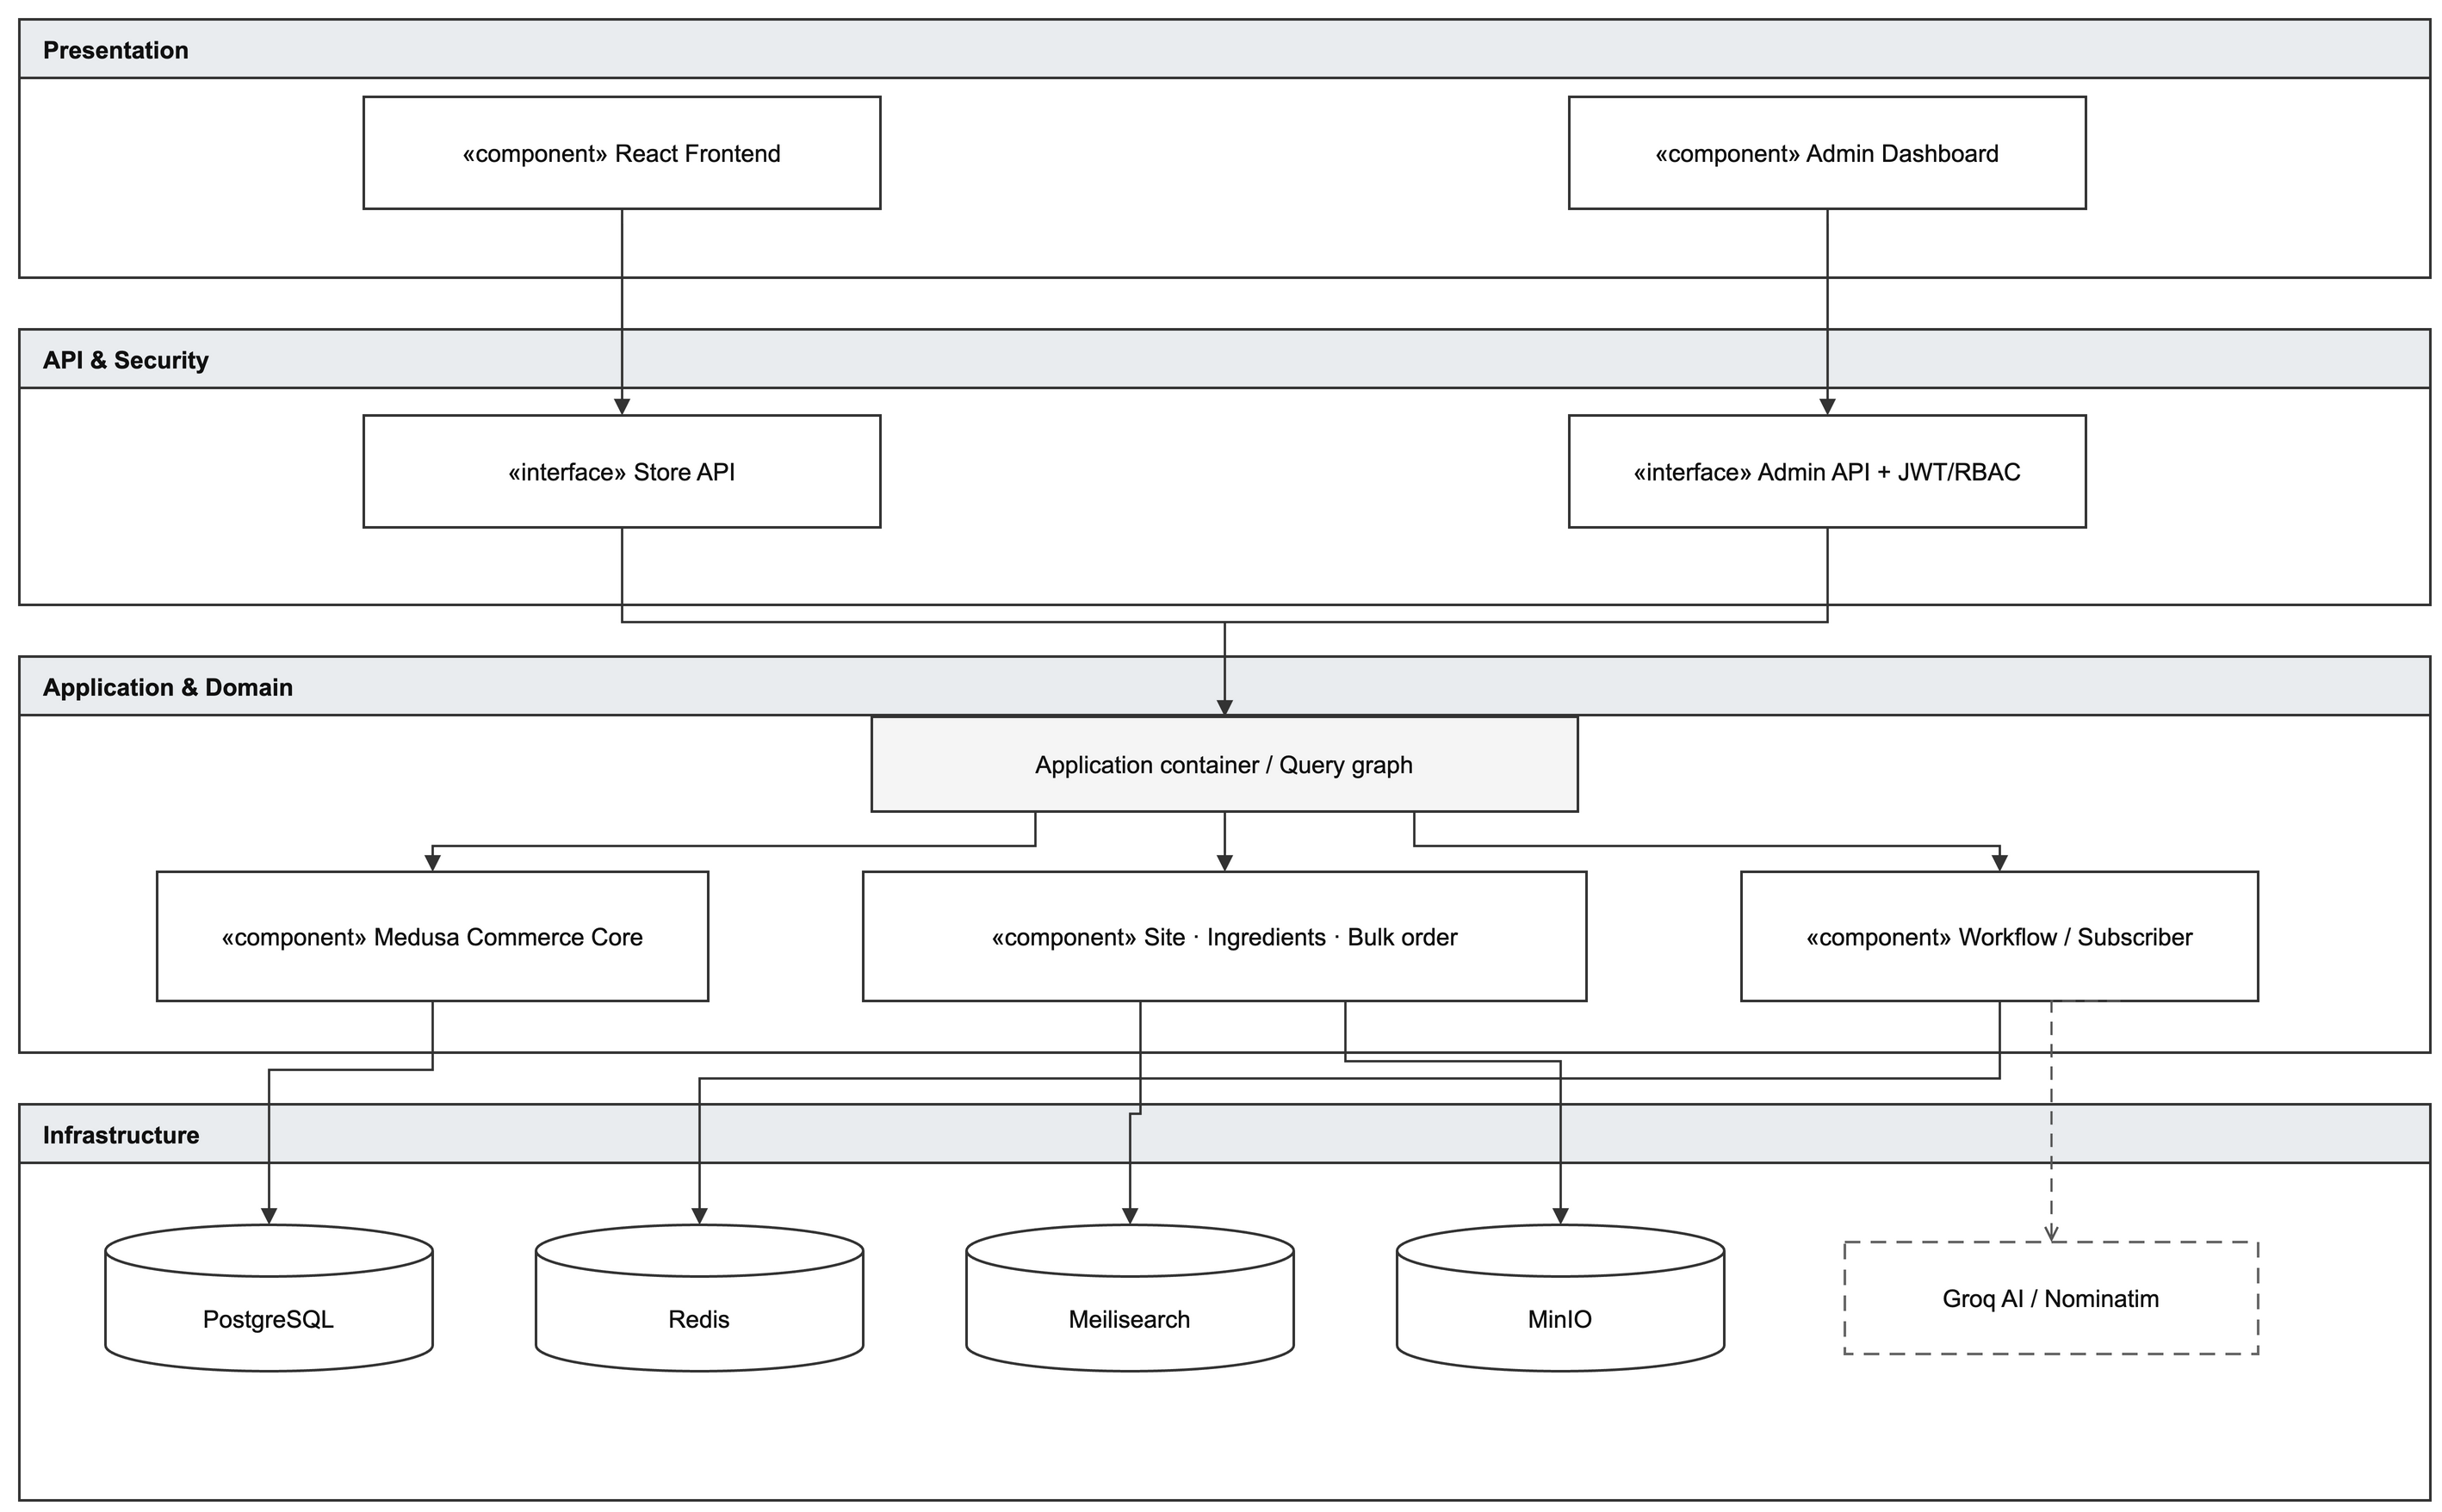
\includegraphics[width=\textwidth,height=0.74\textheight,keepaspectratio]{images/architecture.drawio.png}
  \caption{Kiến trúc logic của Mọng Fruitboxz}
  \label{fig:architecture}
\end{figure}

\section{Thiết Kế Frontend}

\subsection{Tổ chức ứng dụng}

Frontend được xây dựng dưới dạng single-page application. \techterm{React Router} ánh xạ URL tới trang; \techterm{React.lazy} và \techterm{Suspense} tách bundle theo route. Các provider ở cấp ứng dụng quản lý catalog, giỏ hàng, ngôn ngữ, xác thực khách hàng và xác thực quản trị.

\begin{longtable}{@{}p{0.25\textwidth} p{0.67\textwidth}@{}}
  \toprule
  \textbf{Thành phần} & \textbf{Trách nhiệm} \\
  \midrule
  \endhead
  \texttt{apiFetch} & Bọc \texttt{medusa.client.fetch}, tự xử lý timeout, token và cấu trúc response envelope. \\
  \texttt{CatalogContext} & Cung cấp dữ liệu sản phẩm và danh mục cho các trang mua sắm. \\
  \texttt{CartContext} & Quản lý reducer giỏ hàng, localStorage, đồng bộ Redis và thông báo thêm hàng. \\
  \texttt{AuthContext} & Đọc JWT khách hàng, kiểm tra hết hạn và cung cấp trạng thái đăng nhập. \\
  \texttt{AdminAuthContext} & Đăng nhập admin, tải quyền, xử lý 401 và kiểm tra quyền theo chức năng. \\
  \texttt{LanguageContext} & Kết hợp i18next để hỗ trợ nội dung tiếng Việt và tiếng Anh. \\
  \bottomrule
\end{longtable}

\subsection{Nguyên tắc giao tiếp API}

Medusa SDK được cấu hình với backend URL, publishable key và cơ chế lưu JWT. API lõi và API tùy biến đều đi qua một lớp gọi chung để nhất quán timeout và xử lý lỗi. Riêng tìm kiếm có thể gọi Meilisearch trực tiếp khi cấu hình search key phía client; nếu không, giao diện gọi API backend.

\section{Thiết Kế Backend Medusa}

\subsection{Mô-đun lõi và mô-đun mở rộng}

Medusa cung cấp các mô-đun lõi như Product, Pricing, Inventory, Order, Customer, User, Promotion và Region. Dự án đăng ký thêm năm mô-đun:

\begin{itemize}[leftmargin=2em, itemsep=4pt]
  \item \textbf{Site:} banner, cấu hình website, blog, liên hệ và log chatbot.
  \item \textbf{RBAC:} role, permission và ánh xạ quyền của người dùng quản trị.
  \item \textbf{Ingredients:} nguyên liệu, công thức BOM và kiểm tra/trừ tồn kho.
  \item \textbf{Bulk orders:} lưu yêu cầu đặt hàng số lượng lớn.
  \item \textbf{Voting:} điểm và bình luận gắn với khách hàng, sản phẩm.
\end{itemize}

Các module link nối User với Role và Ingredient với InventoryItem mà không đưa khóa ngoại của mô-đun khác trực tiếp vào model tùy biến.

\begin{figure}[H]
  \centering
  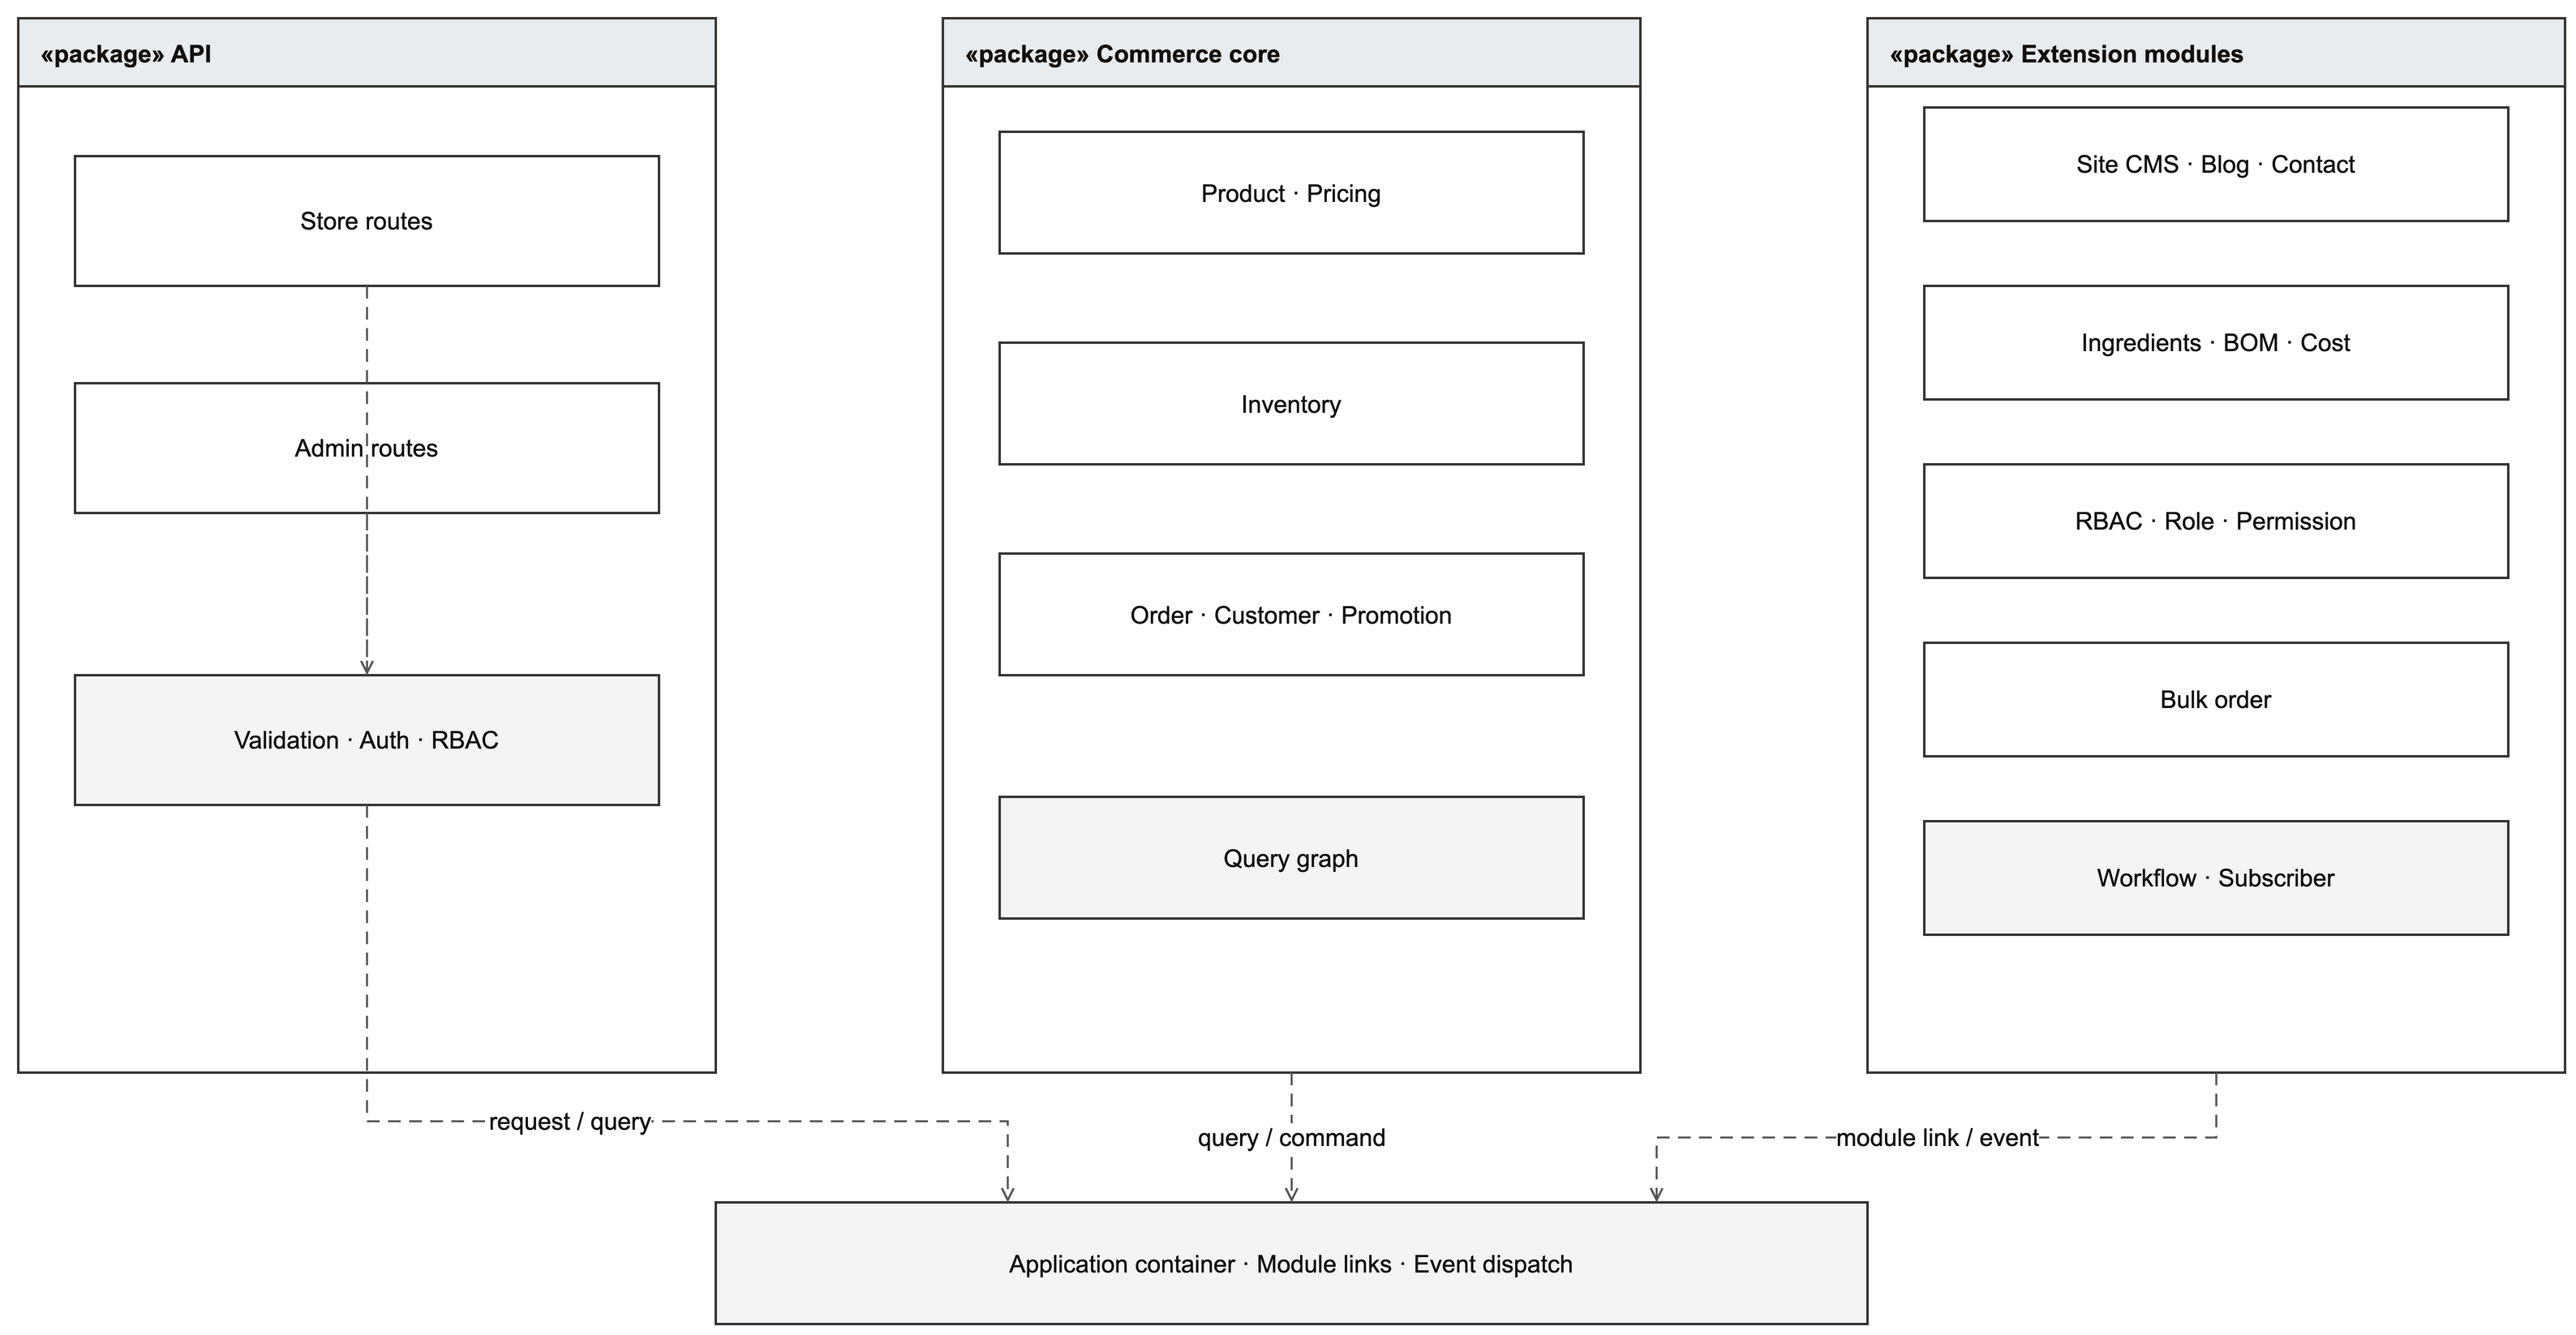
\includegraphics[width=\textwidth,height=0.72\textheight,keepaspectratio]{images/modules.drawio.png}
  \caption{Cấu trúc mô-đun nghiệp vụ và điểm tích hợp}
  \label{fig:module-structure}
\end{figure}

\subsection{API, workflow và subscriber}

API được chia theo hai namespace: \texttt{/store} dành cho khách hàng và \texttt{/admin} dành cho vận hành. Middleware chung thực hiện xác thực, RBAC, validation và chuẩn hóa response. Workflow đã được sử dụng cho luồng tạo contact message. Các thay đổi sản phẩm và đơn hàng được xử lý tiếp bằng subscriber:

\begin{itemize}[leftmargin=2em, itemsep=3pt]
  \item Sản phẩm tạo/cập nhật/xóa sẽ đồng bộ tài liệu tương ứng trong Meilisearch và vô hiệu cache.
  \item Danh mục thay đổi sẽ xóa cache danh mục và cache tìm kiếm.
  \item Đơn được tạo sẽ phát sự kiện \texttt{order.placed}; subscriber trừ tồn nguyên liệu và chuẩn bị email xác nhận.
\end{itemize}

\section{Luồng Checkout}

\subsection{Biểu đồ hoạt động}

Biểu đồ hoạt động trong Hình~\ref{fig:checkout-activity} tách trách nhiệm thành bốn swimlane. Frontend chỉ kiểm tra dữ liệu ở mức giao diện; Checkout API xác minh lại dữ liệu tin cậy; dịch vụ nghiệp vụ chịu trách nhiệm tồn kho, phí giao hàng và khuyến mãi. Hai nút quyết định thể hiện rõ đường thành công và đường quay lại sửa dữ liệu.

\begin{figure}[H]
  \centering
  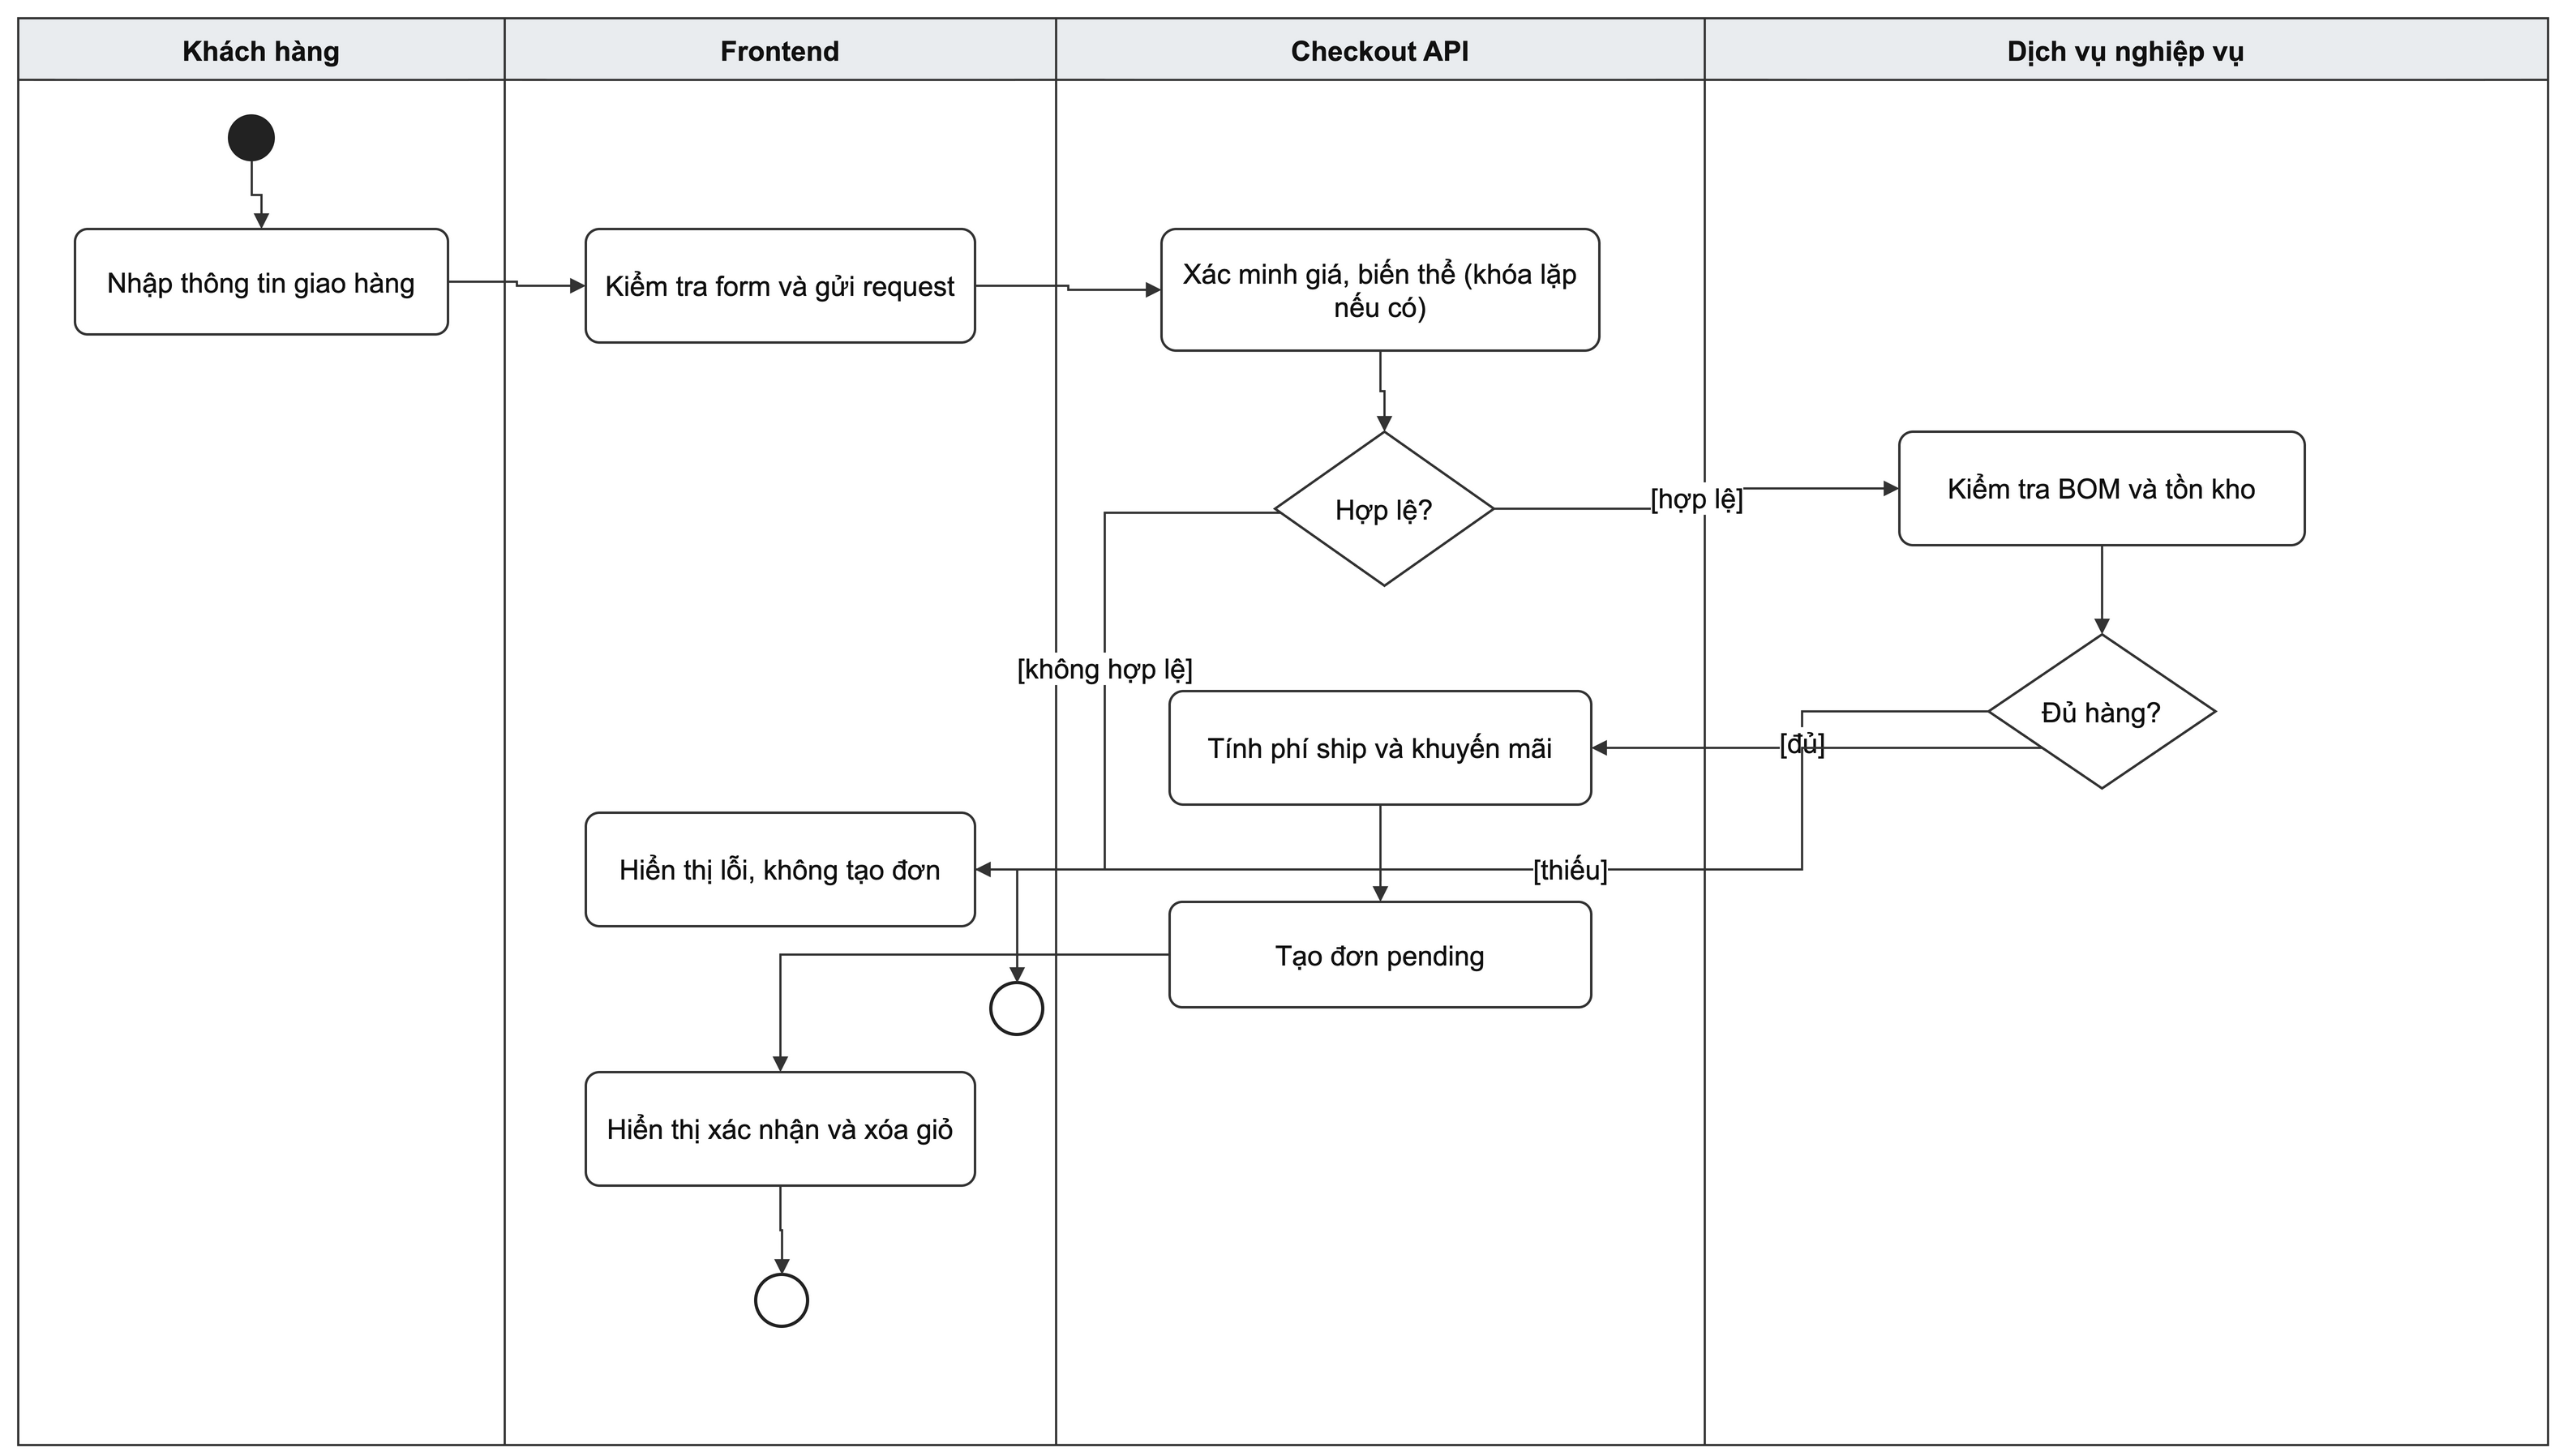
\includegraphics[width=\textwidth,height=0.76\textheight,keepaspectratio]{images/activity-checkout.drawio.png}
  \caption{Biểu đồ hoạt động của quy trình checkout}
  \label{fig:checkout-activity}
\end{figure}

\subsection{Biểu đồ trình tự}

\begin{figure}[H]
  \centering
  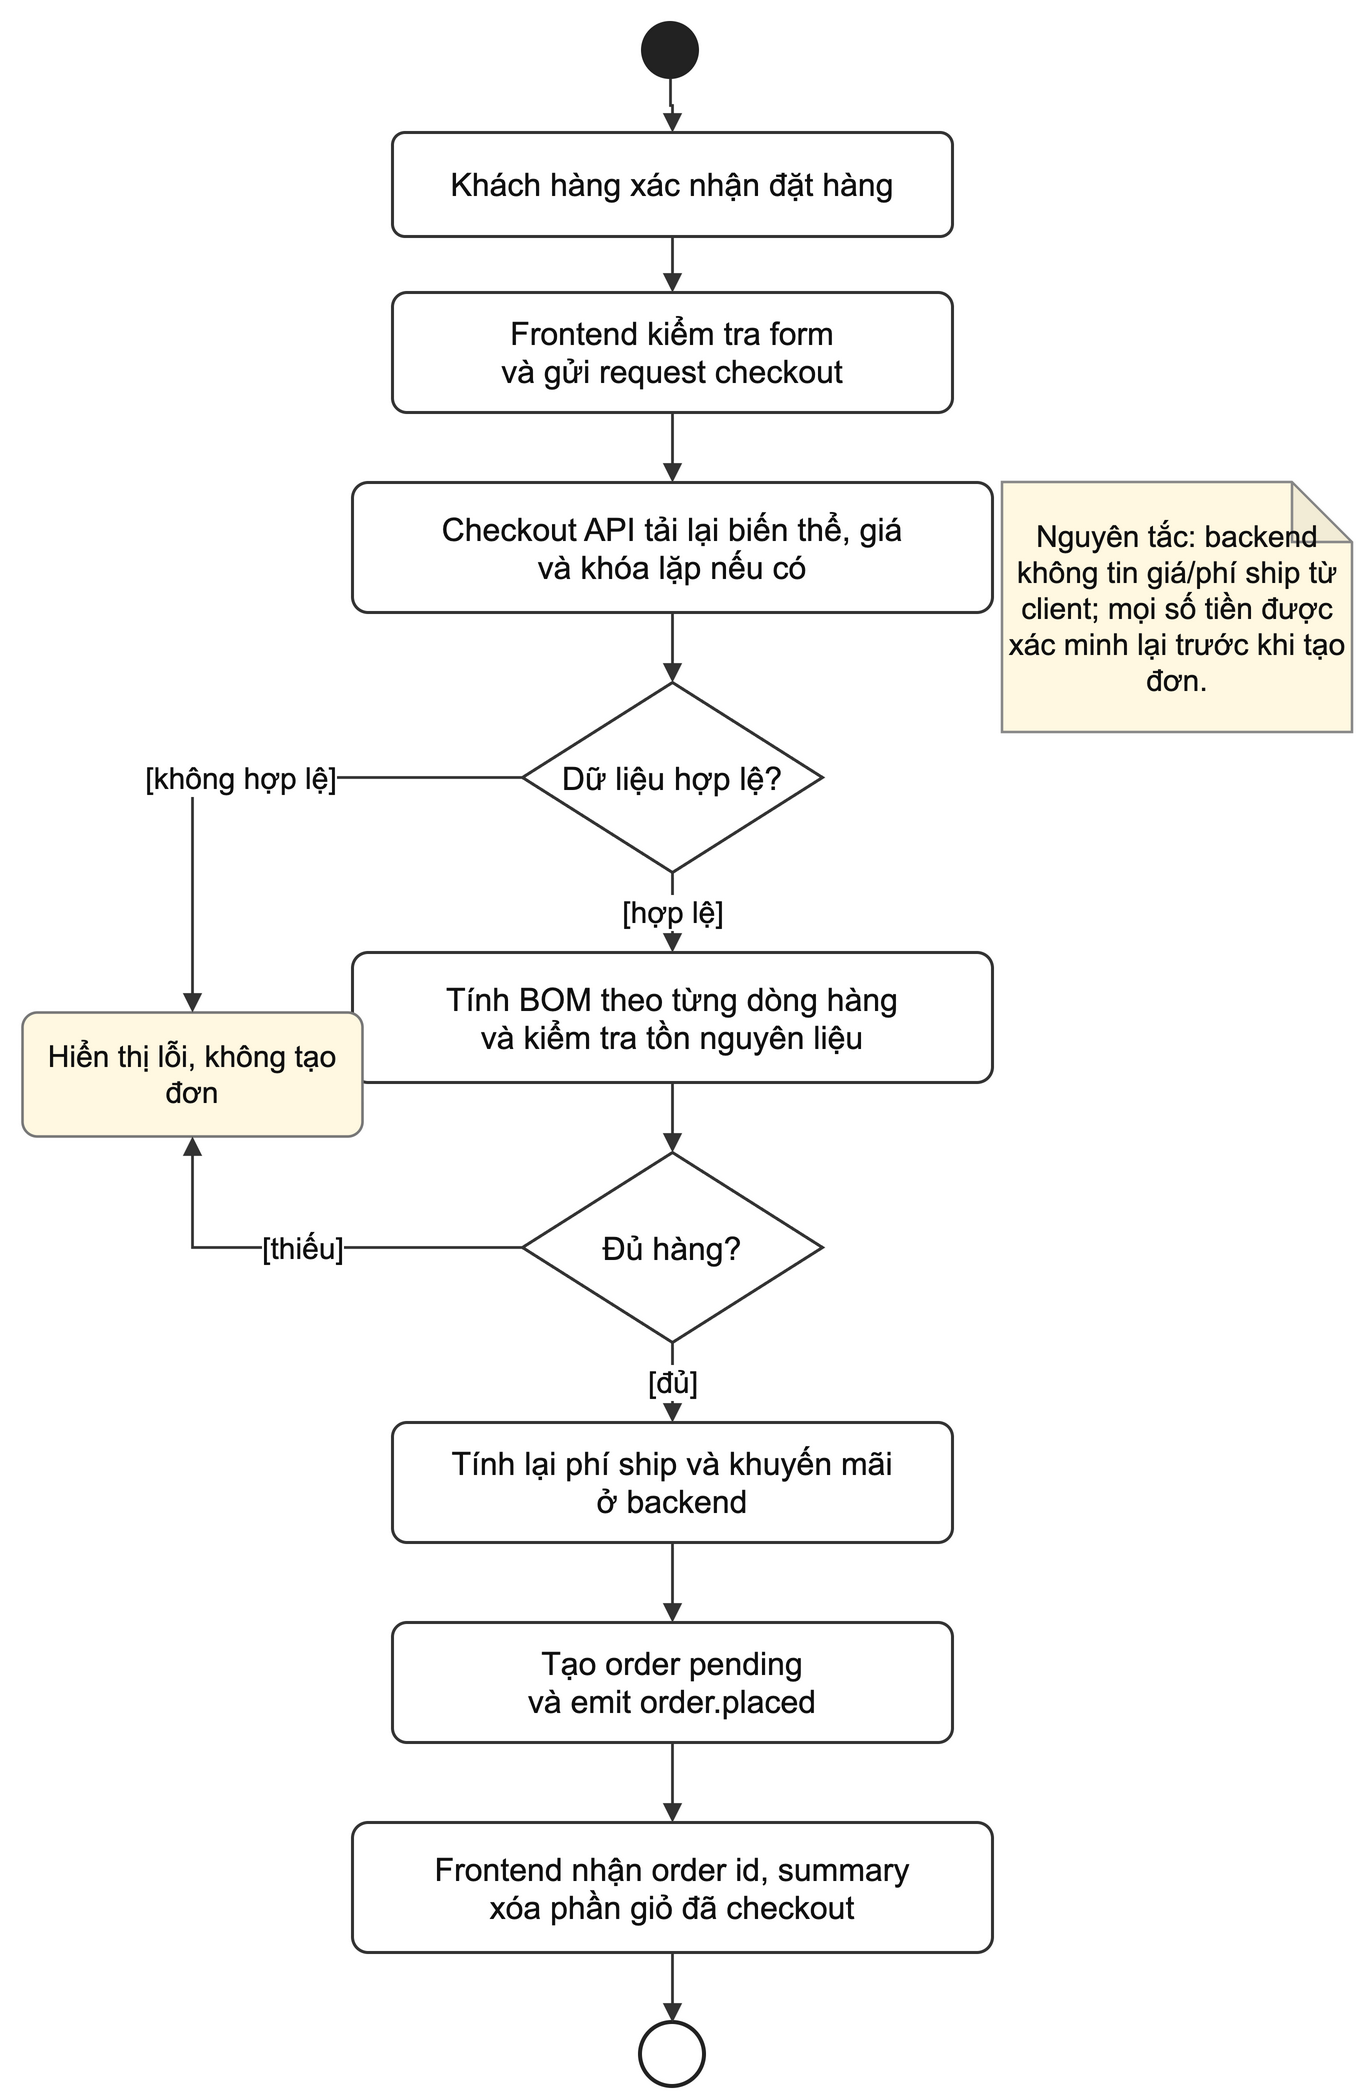
\includegraphics[width=\textwidth,height=0.76\textheight,keepaspectratio]{images/checkout-sequence.drawio.png}
  \caption{Biểu đồ trình tự của luồng xử lý đặt hàng}
  \label{fig:checkout-flow}
\end{figure}

Điểm quan trọng của thiết kế là backend không chấp nhận giá do trình duyệt gửi. Tuy nhiên, route checkout hiện tạo đơn trực tiếp qua service và tự phát sự kiện, tức chưa sử dụng đầy đủ workflow có compensation của Medusa. Đây là điểm cần tái cấu trúc để đảm bảo rollback khi một bước sau tạo đơn thất bại.

\section{Mô Hình Lớp Miền}

Hình~\ref{fig:domain-class} giữ lại các lớp có ảnh hưởng trực tiếp đến catalog, công thức nguyên liệu, đơn hàng và RBAC. Product sở hữu nhiều ProductVariant; mỗi biến thể có nhiều RecipeItem nối tới Ingredient; Ingredient được ánh xạ tới một InventoryItem để theo dõi lượng tồn. Order sở hữu các dòng OrderLineItem và mỗi dòng tham chiếu đúng một biến thể tại thời điểm mua.

\begin{figure}[H]
  \centering
  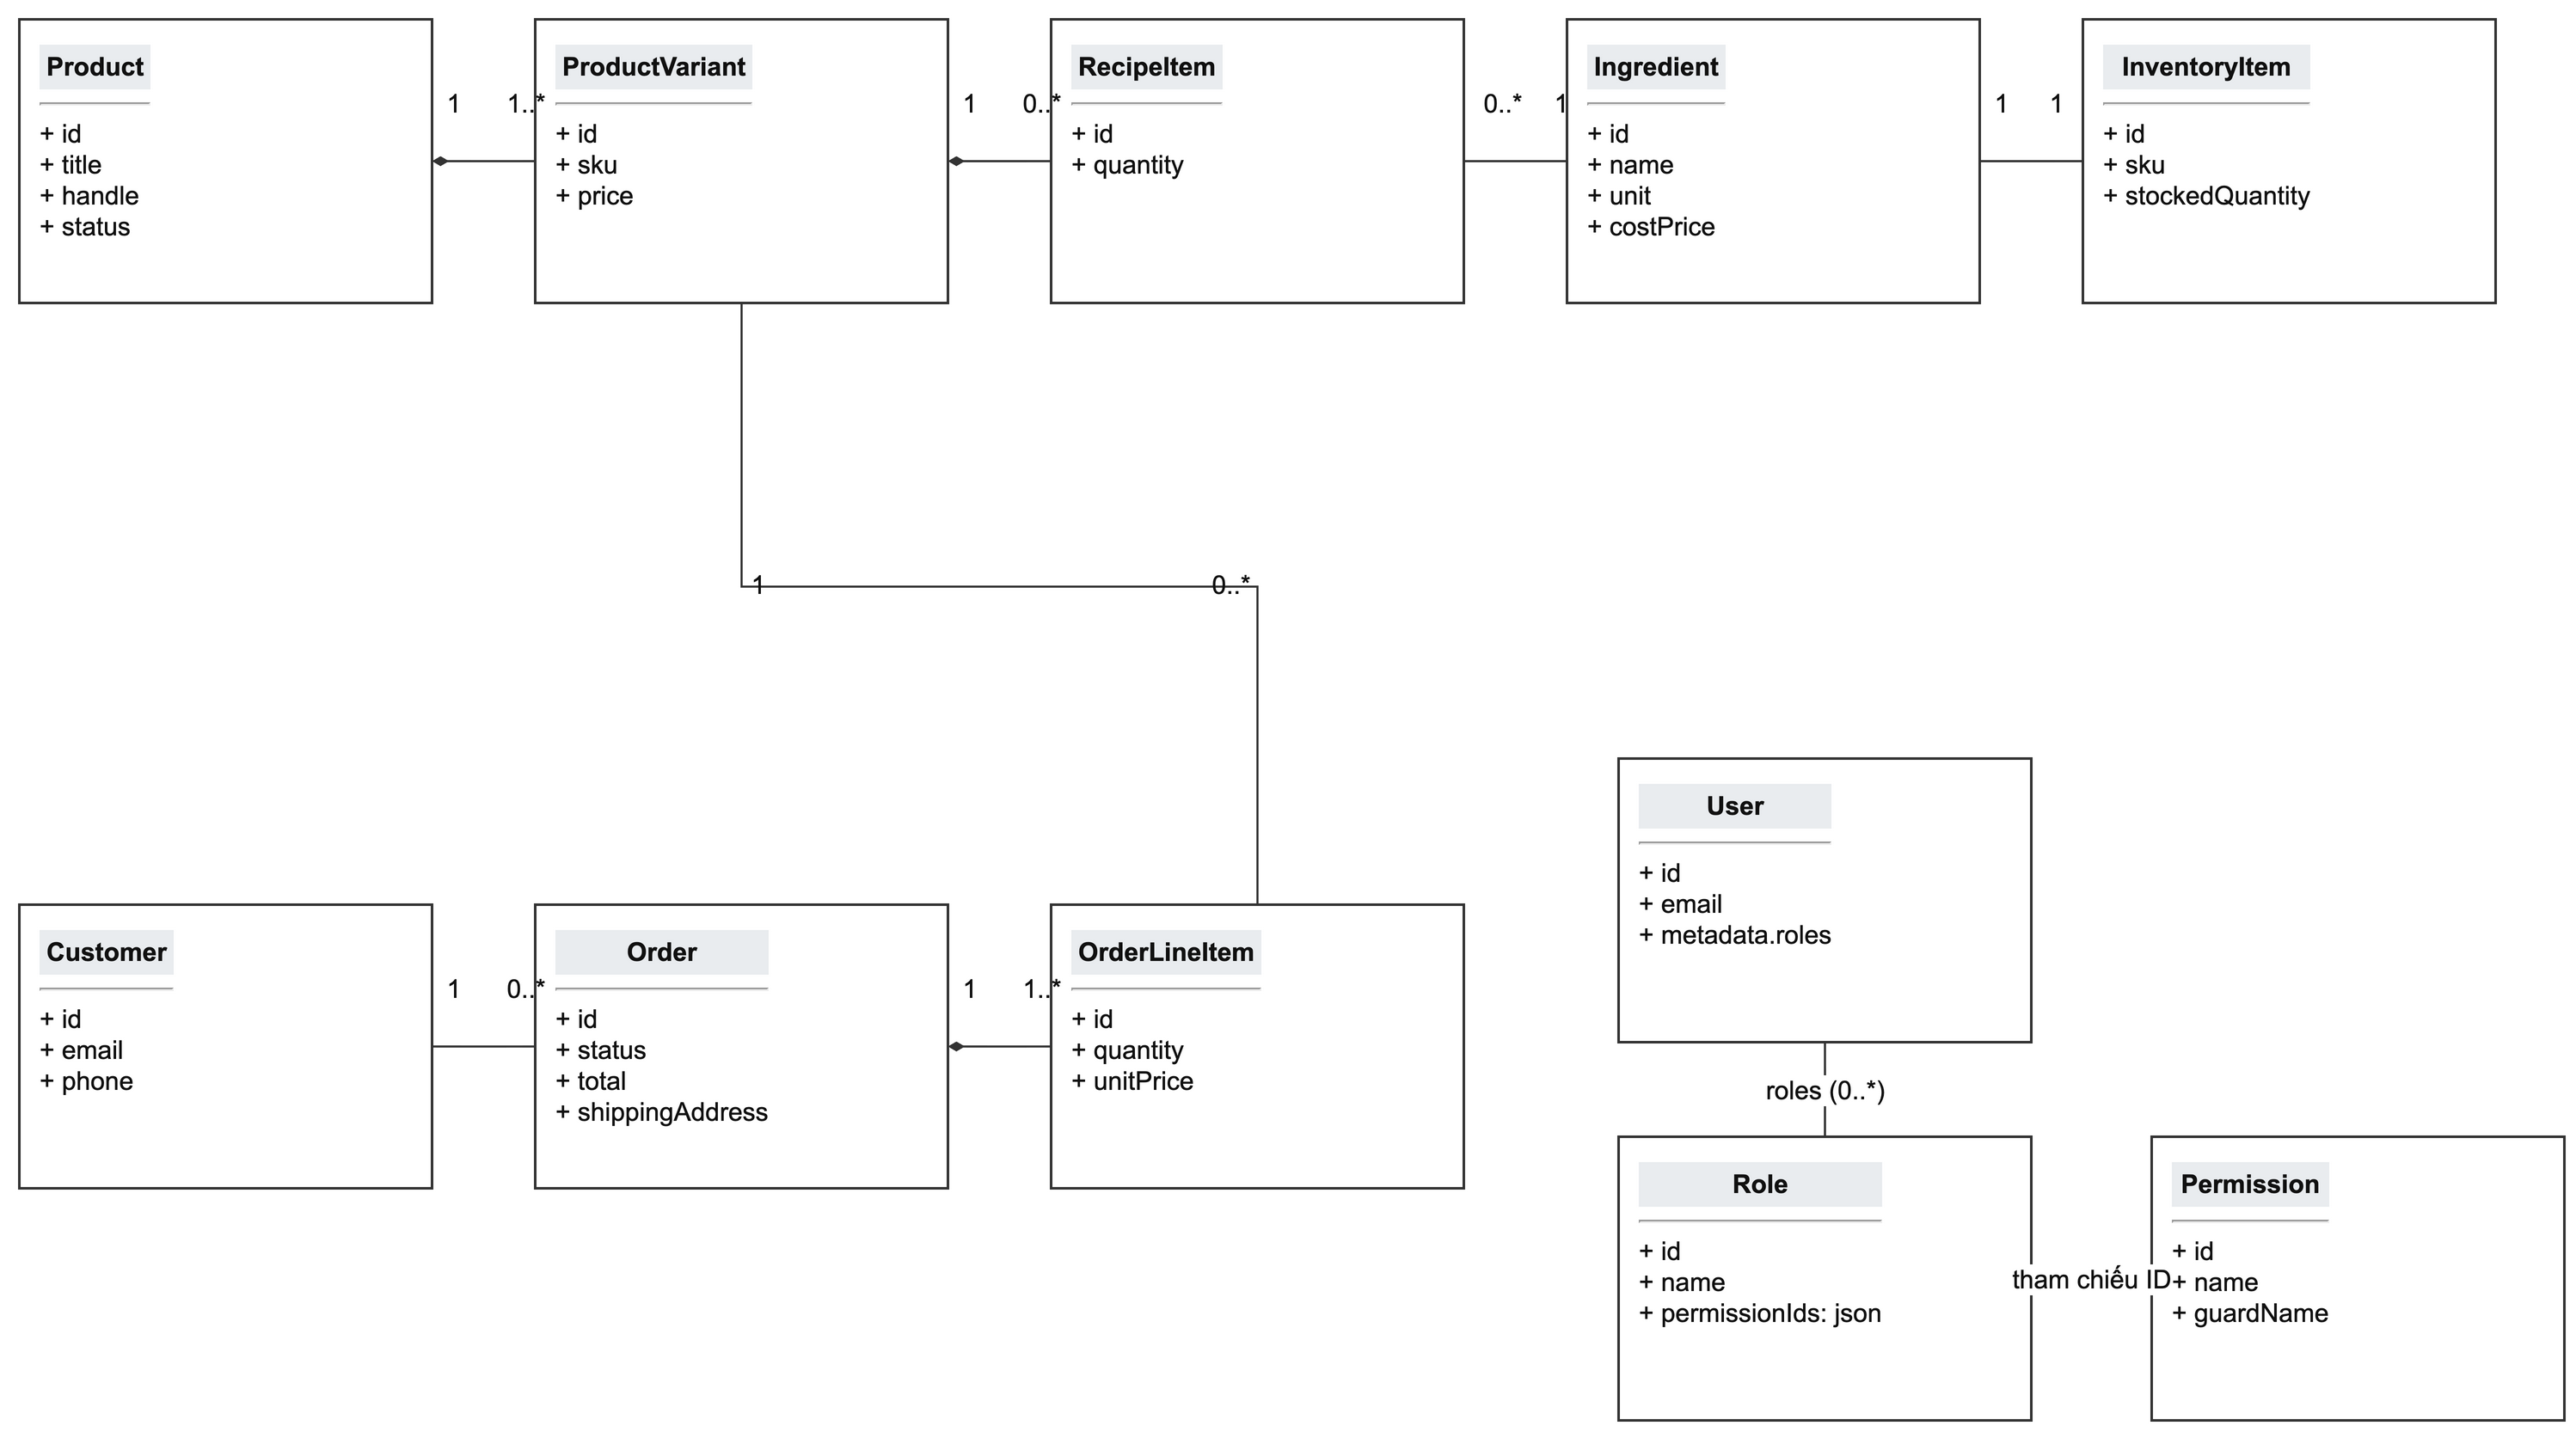
\includegraphics[width=\textwidth,height=0.78\textheight,keepaspectratio]{images/domain-class.drawio.png}
  \caption{Biểu đồ lớp miền nghiệp vụ chính}
  \label{fig:domain-class}
\end{figure}

Các bội số trên quan hệ giúp kiểm tra mô hình trước khi cài đặt. Ví dụ, một Order không nên tồn tại mà không có OrderLineItem; một ProductVariant có thể chưa được cấu hình công thức; Role và Permission có quan hệ nhiều--nhiều. Các lớp trong sơ đồ là mô hình logic, không đồng nghĩa mỗi quan hệ phải được cài bằng khóa ngoại trực tiếp vì Medusa sử dụng module link để bảo toàn ranh giới mô-đun.

\section{Tìm Kiếm và Chatbot}

Tài liệu tìm kiếm chứa tên, mô tả, slug, danh mục, mức giá, giá nhỏ nhất/lớn nhất, ảnh và trạng thái tồn. Subscriber giữ chỉ mục đồng bộ với catalog. Khi tìm kiếm chính không hoạt động, backend xây tài liệu từ Query API và lọc tại ứng dụng.

Chatbot sử dụng mô hình retrieval-augmented generation ở mức đơn giản: truy vấn FAQ và sản phẩm liên quan, tạo system prompt có giới hạn quyền hạn, sau đó gọi Groq. Response được cache 12 giờ theo câu hỏi. Log lưu message đã chuẩn hóa, chế độ phản hồi, trạng thái resolved và số gợi ý; nhờ đó quản trị viên có thể bổ sung FAQ cho câu hỏi chưa được giải quyết.

\begin{figure}[H]
  \centering
  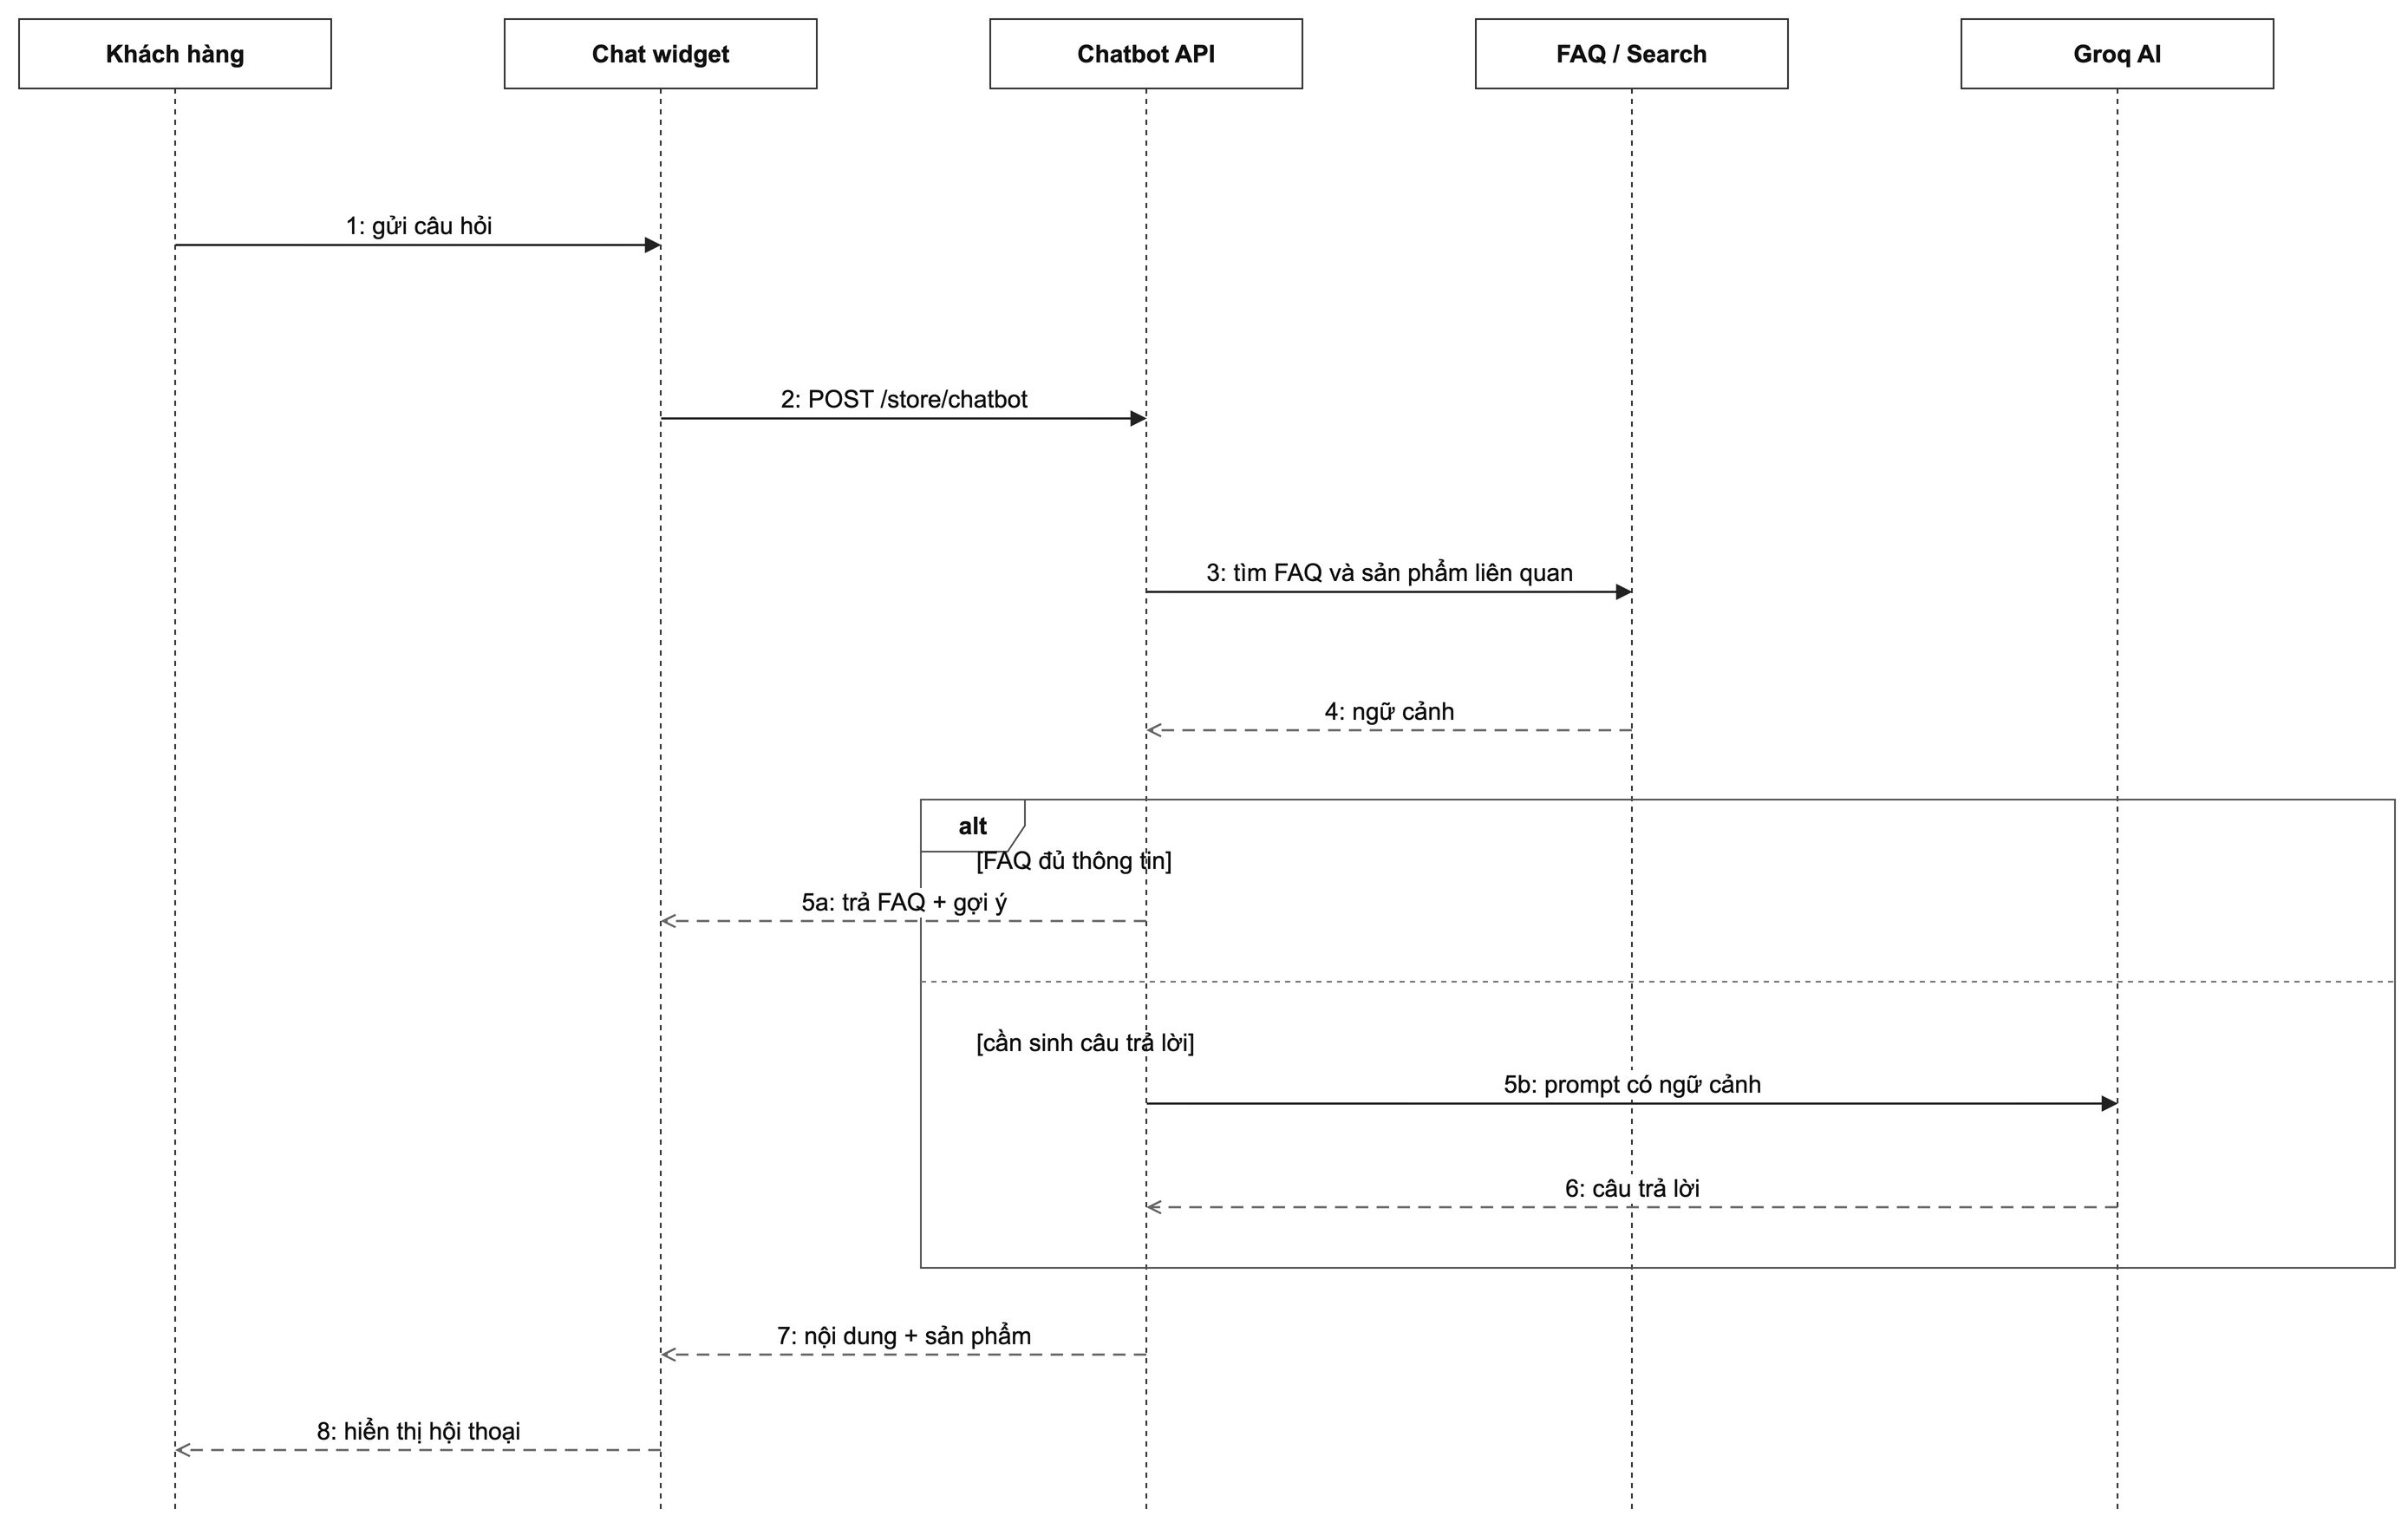
\includegraphics[width=\textwidth,height=0.74\textheight,keepaspectratio]{images/chatbot-sequence.drawio.png}
  \caption{Biểu đồ trình tự của chatbot tư vấn sản phẩm}
  \label{fig:chatbot-sequence}
\end{figure}

\section{Bảo Mật}

\begin{itemize}[leftmargin=2em, itemsep=4pt]
  \item JWT tách riêng cho khách hàng và người dùng quản trị; token hết hạn bị xóa khỏi localStorage.
  \item API admin sử dụng middleware xác thực và RBAC; quyền được kiểm tra lại ở backend, không chỉ dựa vào việc ẩn menu.
  \item Checkout khách được cho phép nhưng không tự liên kết với customer có cùng email, tránh chiếm quyền lịch sử đơn.
  \item Chatbot có rate limit, phạm vi dữ liệu hạn chế và quy tắc chống prompt injection cơ bản.
  \item CORS, JWT secret, cookie secret và khóa dịch vụ được cấu hình bằng biến môi trường.
\end{itemize}

\section{Vòng Đời Đơn Hàng}

Trạng thái đơn được mô hình hóa riêng để tránh cập nhật tùy ý từ giao diện quản trị. Luồng chuẩn đi từ \texttt{pending} tới \texttt{confirmed}, \texttt{processing}, \texttt{shipping} và \texttt{completed}. Hủy đơn chỉ hợp lệ trước khi giao; lỗi giao vận hoặc xử lý có thể chuyển sang \texttt{failed} và được retry có kiểm soát.

\begin{figure}[H]
  \centering
  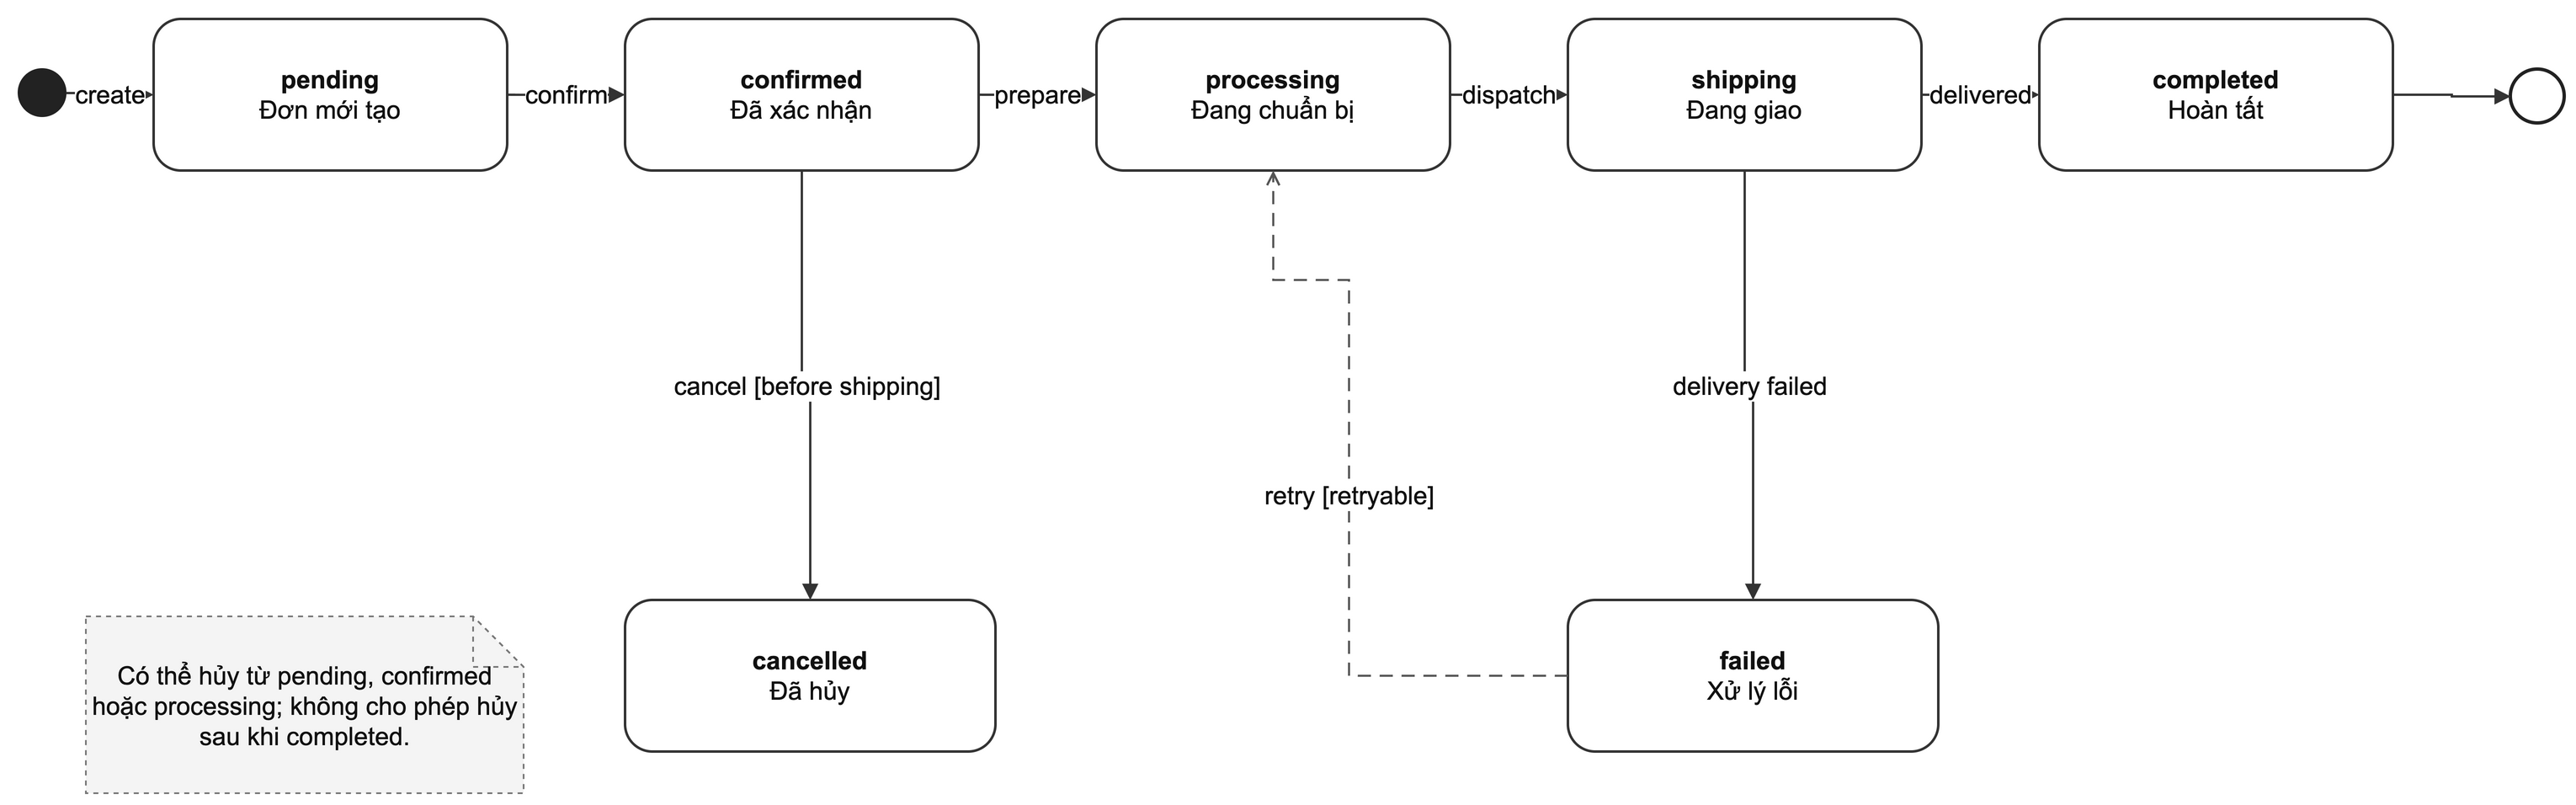
\includegraphics[width=\textwidth,height=0.55\textheight,keepaspectratio]{images/order-state.drawio.png}
  \caption{Biểu đồ trạng thái đơn hàng}
  \label{fig:order-state}
\end{figure}

Mỗi chuyển tiếp nên được thực hiện qua một command hoặc workflow có kiểm tra trạng thái nguồn, quyền người thao tác và tác dụng phụ tương ứng. Cách này ngăn các chuyển tiếp vô nghĩa như đưa đơn đã hoàn tất quay lại xử lý, đồng thời tạo điểm rõ ràng để phát sự kiện, ghi audit log và gửi thông báo.

\section{Mô Hình Triển Khai}

Trong môi trường phát triển, Docker Compose chạy bốn dịch vụ: PostgreSQL cổng 5432, Redis cổng 6379, Meilisearch cổng 7700 và MinIO (S3 API được ánh xạ ra cổng 9001, console cổng 9002). Backend chạy ở cổng 9000; frontend Vite hiện cấu hình cổng 5173 và proxy các đường dẫn \texttt{/auth}, \texttt{/store}, \texttt{/admin}, \texttt{/media} tới backend.

\begin{figure}[H]
  \centering
  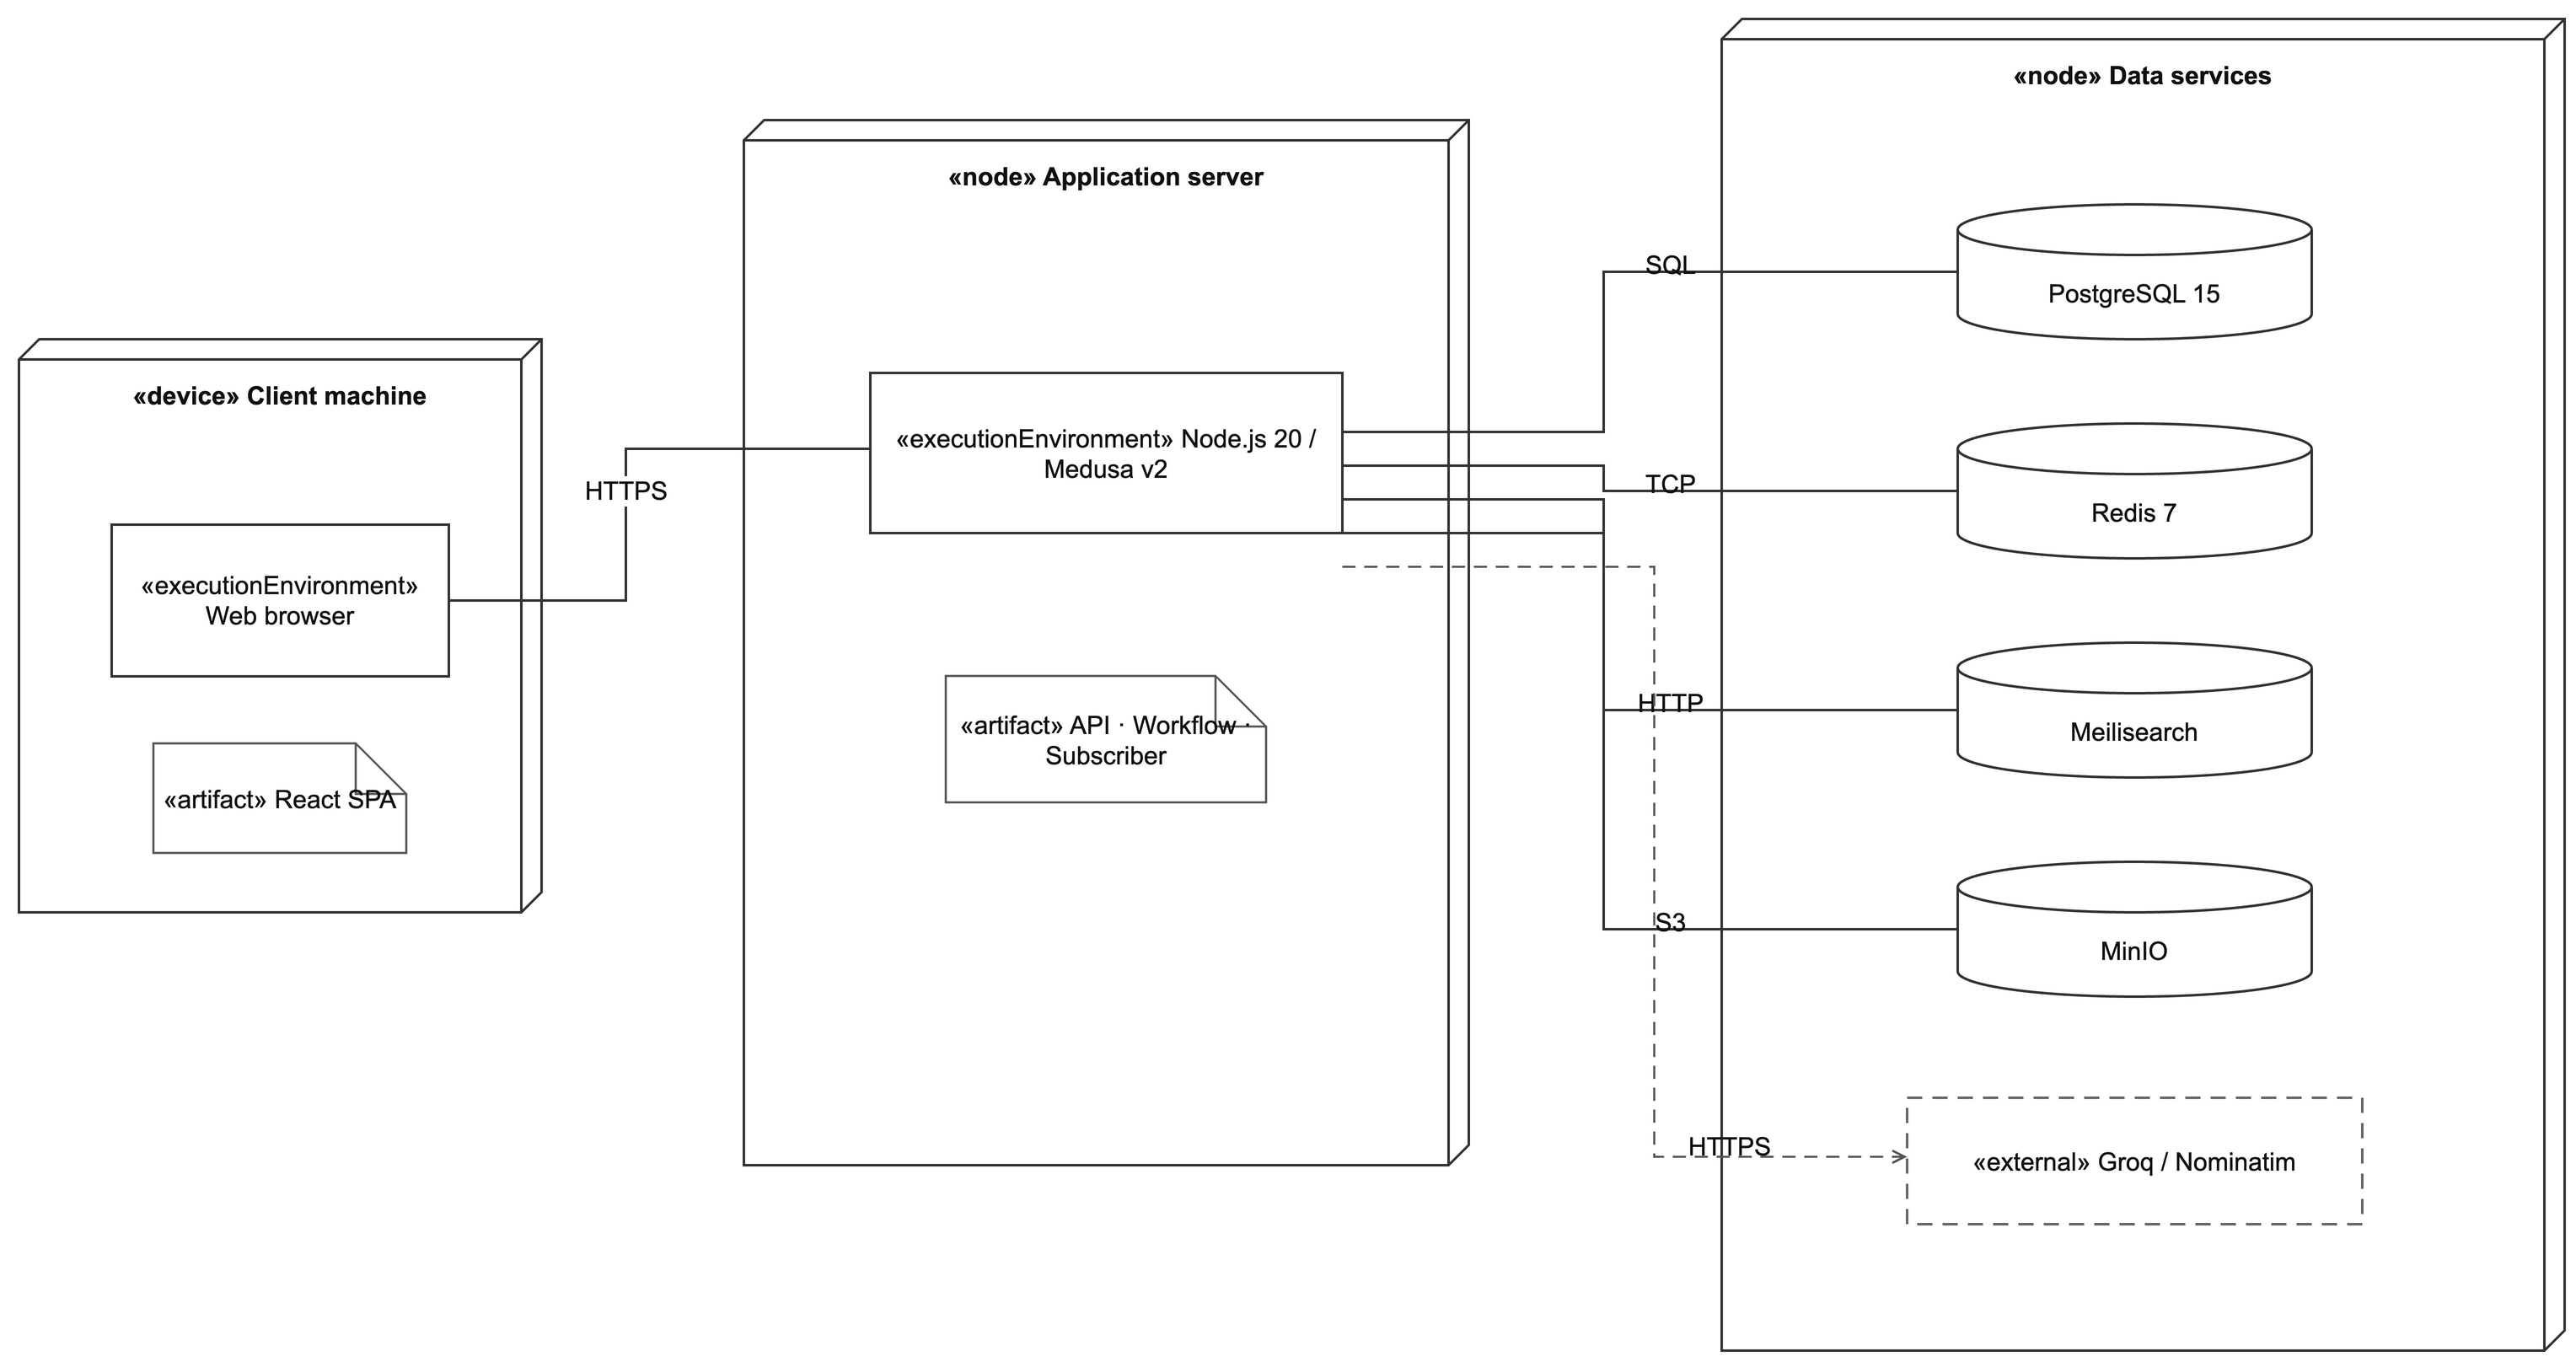
\includegraphics[width=\textwidth,height=0.70\textheight,keepaspectratio]{images/deployment.drawio.png}
  \caption{Mô hình triển khai và các dịch vụ tích hợp}
  \label{fig:deployment}
\end{figure}

Ở production, cần tách secret khỏi mã nguồn, bật HTTPS, giới hạn truy cập Meilisearch/MinIO, cấu hình Redis thật cho cache/event bus và đặt reverse proxy trước hai ứng dụng.

% ============================================================
%  04_csdl.tex – Chương 4: Thiết kế dữ liệu
% ============================================================
\chapter{Thiết Kế Dữ Liệu}

\section{Tổng Quan}

Hệ thống sử dụng PostgreSQL 15. Phần lớn bảng thương mại điện tử được Medusa quản lý thông qua module và migration; dự án bổ sung các bảng riêng cho nội dung website, phân quyền, nguyên liệu và yêu cầu mua số lượng lớn. Vì Medusa khuyến khích cô lập mô-đun, quan hệ giữa mô-đun lõi và mô-đun tùy biến được khai báo bằng module link.

Ngoài cơ sở dữ liệu quan hệ, hệ thống còn dùng Redis cho dữ liệu tạm thời, Meilisearch cho chỉ mục tìm kiếm và MinIO cho tệp nhị phân. Ba thành phần này không thay thế PostgreSQL mà phục vụ các kiểu truy cập chuyên biệt.

\section{Nhóm Thực Thể Lõi Của Medusa}

\begin{longtable}{@{}p{0.22\textwidth} p{0.28\textwidth} p{0.42\textwidth}@{}}
  \toprule
  \textbf{Miền} & \textbf{Thực thể tiêu biểu} & \textbf{Ý nghĩa} \\
  \midrule
  \endhead
  Catalog & Product, ProductVariant, ProductCategory, ProductImage & Thông tin sản phẩm, biến thể, danh mục và ảnh. \\
  Giá bán & Price, PriceSet, Region & Giá theo biến thể, tiền tệ và khu vực bán hàng. \\
  Kho & InventoryItem, InventoryLevel, StockLocation & Số lượng hàng hoặc nguyên liệu tại từng vị trí kho. \\
  Khách hàng & Customer, AuthIdentity & Hồ sơ khách và định danh đăng nhập. \\
  Đơn hàng & Order, OrderItem, OrderAddress & Đơn, dòng hàng, địa chỉ và metadata vận hành. \\
  Khuyến mãi & Promotion, ApplicationMethod, Campaign & Mã giảm giá, cách tính và giới hạn chương trình. \\
  Quản trị & User, AuthIdentity & Người dùng nội bộ và thông tin xác thực. \\
  \bottomrule
\end{longtable}

\section{Các Model Tùy Biến}

\subsection{Mô-đun Site}

\begin{longtable}{@{}p{0.23\textwidth} p{0.31\textwidth} p{0.38\textwidth}@{}}
  \toprule
  \textbf{Model} & \textbf{Thuộc tính chính} & \textbf{Mục đích} \\
  \midrule
  \endhead
  \texttt{site\_banner} & title, subtitle, image, link, order, active & Banner động trên frontend, có thứ tự và trạng thái. \\
  \texttt{site\_setting} & key, value (JSON) & Cấu hình tổng quát như giao hàng, chính sách, hotline và chatbot. \\
  \shortstack[l]{\texttt{site\_blog\_}\\\texttt{category}} & name, slug, description & Danh mục bài viết. \\
  \texttt{site\_blog\_post} & title, slug, excerpt, content, image, author, category, published, published\_at & Nội dung blog và trạng thái xuất bản. \\
  \shortstack[l]{\texttt{site\_contact\_}\\\texttt{message}} & name, email, phone, message, status & Yêu cầu liên hệ từ khách hàng. \\
  \shortstack[l]{\texttt{site\_chatbot\_}\\\texttt{question\_log}} & message, normalized\_message, response\_mode, resolved, metadata & Theo dõi chất lượng câu trả lời chatbot. \\
  \bottomrule
\end{longtable}

\subsection{Mô-đun RBAC}

\begin{longtable}{@{}p{0.22\textwidth} p{0.33\textwidth} p{0.37\textwidth}@{}}
  \toprule
  \textbf{Model} & \textbf{Thuộc tính chính} & \textbf{Mục đích} \\
  \midrule
  \endhead
  \texttt{role} & name, description, guard\_name, is\_default, permissions (JSON) & Nhóm quyền của người dùng quản trị. \\
  \texttt{permission} & name, description, guard\_name & Quyền nguyên tử dạng \texttt{module.action}. \\
  \bottomrule
\end{longtable}

Danh sách ID role hiện được lưu trong metadata của User và đồng thời dự án có module link User--Role. Mỗi role lưu mảng ID permission trong trường JSON. Cách này linh hoạt khi seed dữ liệu nhưng cần chuẩn hóa để tránh hai nguồn liên kết cùng tồn tại lâu dài.

\subsection{Mô-đun Ingredients}

\begin{longtable}{@{}p{0.22\textwidth} p{0.33\textwidth} p{0.37\textwidth}@{}}
  \toprule
  \textbf{Model} & \textbf{Thuộc tính chính} & \textbf{Mục đích} \\
  \midrule
  \endhead
  \texttt{ingredient} & name, type, unit, cost\_price & Nguyên liệu như trái cây, sốt, sữa chua hoặc thành phần khác. \\
  \texttt{recipe\_item} & variant\_id, quantity, ingredient & Định mức một nguyên liệu cho một biến thể sản phẩm. \\
  \bottomrule
\end{longtable}

Một Ingredient liên kết một-một với InventoryItem của Medusa. Khi đặt $q$ sản phẩm, lượng nguyên liệu $i$ cần dùng được tính theo:

\begin{equation}
  D_i = \sum_{v \in V} q_v \times r_{v,i}
\end{equation}

trong đó $q_v$ là số lượng biến thể $v$ trong đơn và $r_{v,i}$ là định mức nguyên liệu $i$ trong công thức của biến thể đó. Đơn chỉ được tạo khi tồn khả dụng của mọi nguyên liệu không nhỏ hơn $D_i$.

\subsection{Các mô-đun khác}

\begin{itemize}[leftmargin=2em, itemsep=4pt]
  \item \texttt{bulk\_order}: lưu tên công ty, email, điện thoại, ngày yêu cầu, ghi chú và trạng thái của đơn số lượng lớn.
\end{itemize}

\section{Quan Hệ Dữ Liệu}

\begin{diagramcanvas}
\begin{figure}[H]
  \centering
  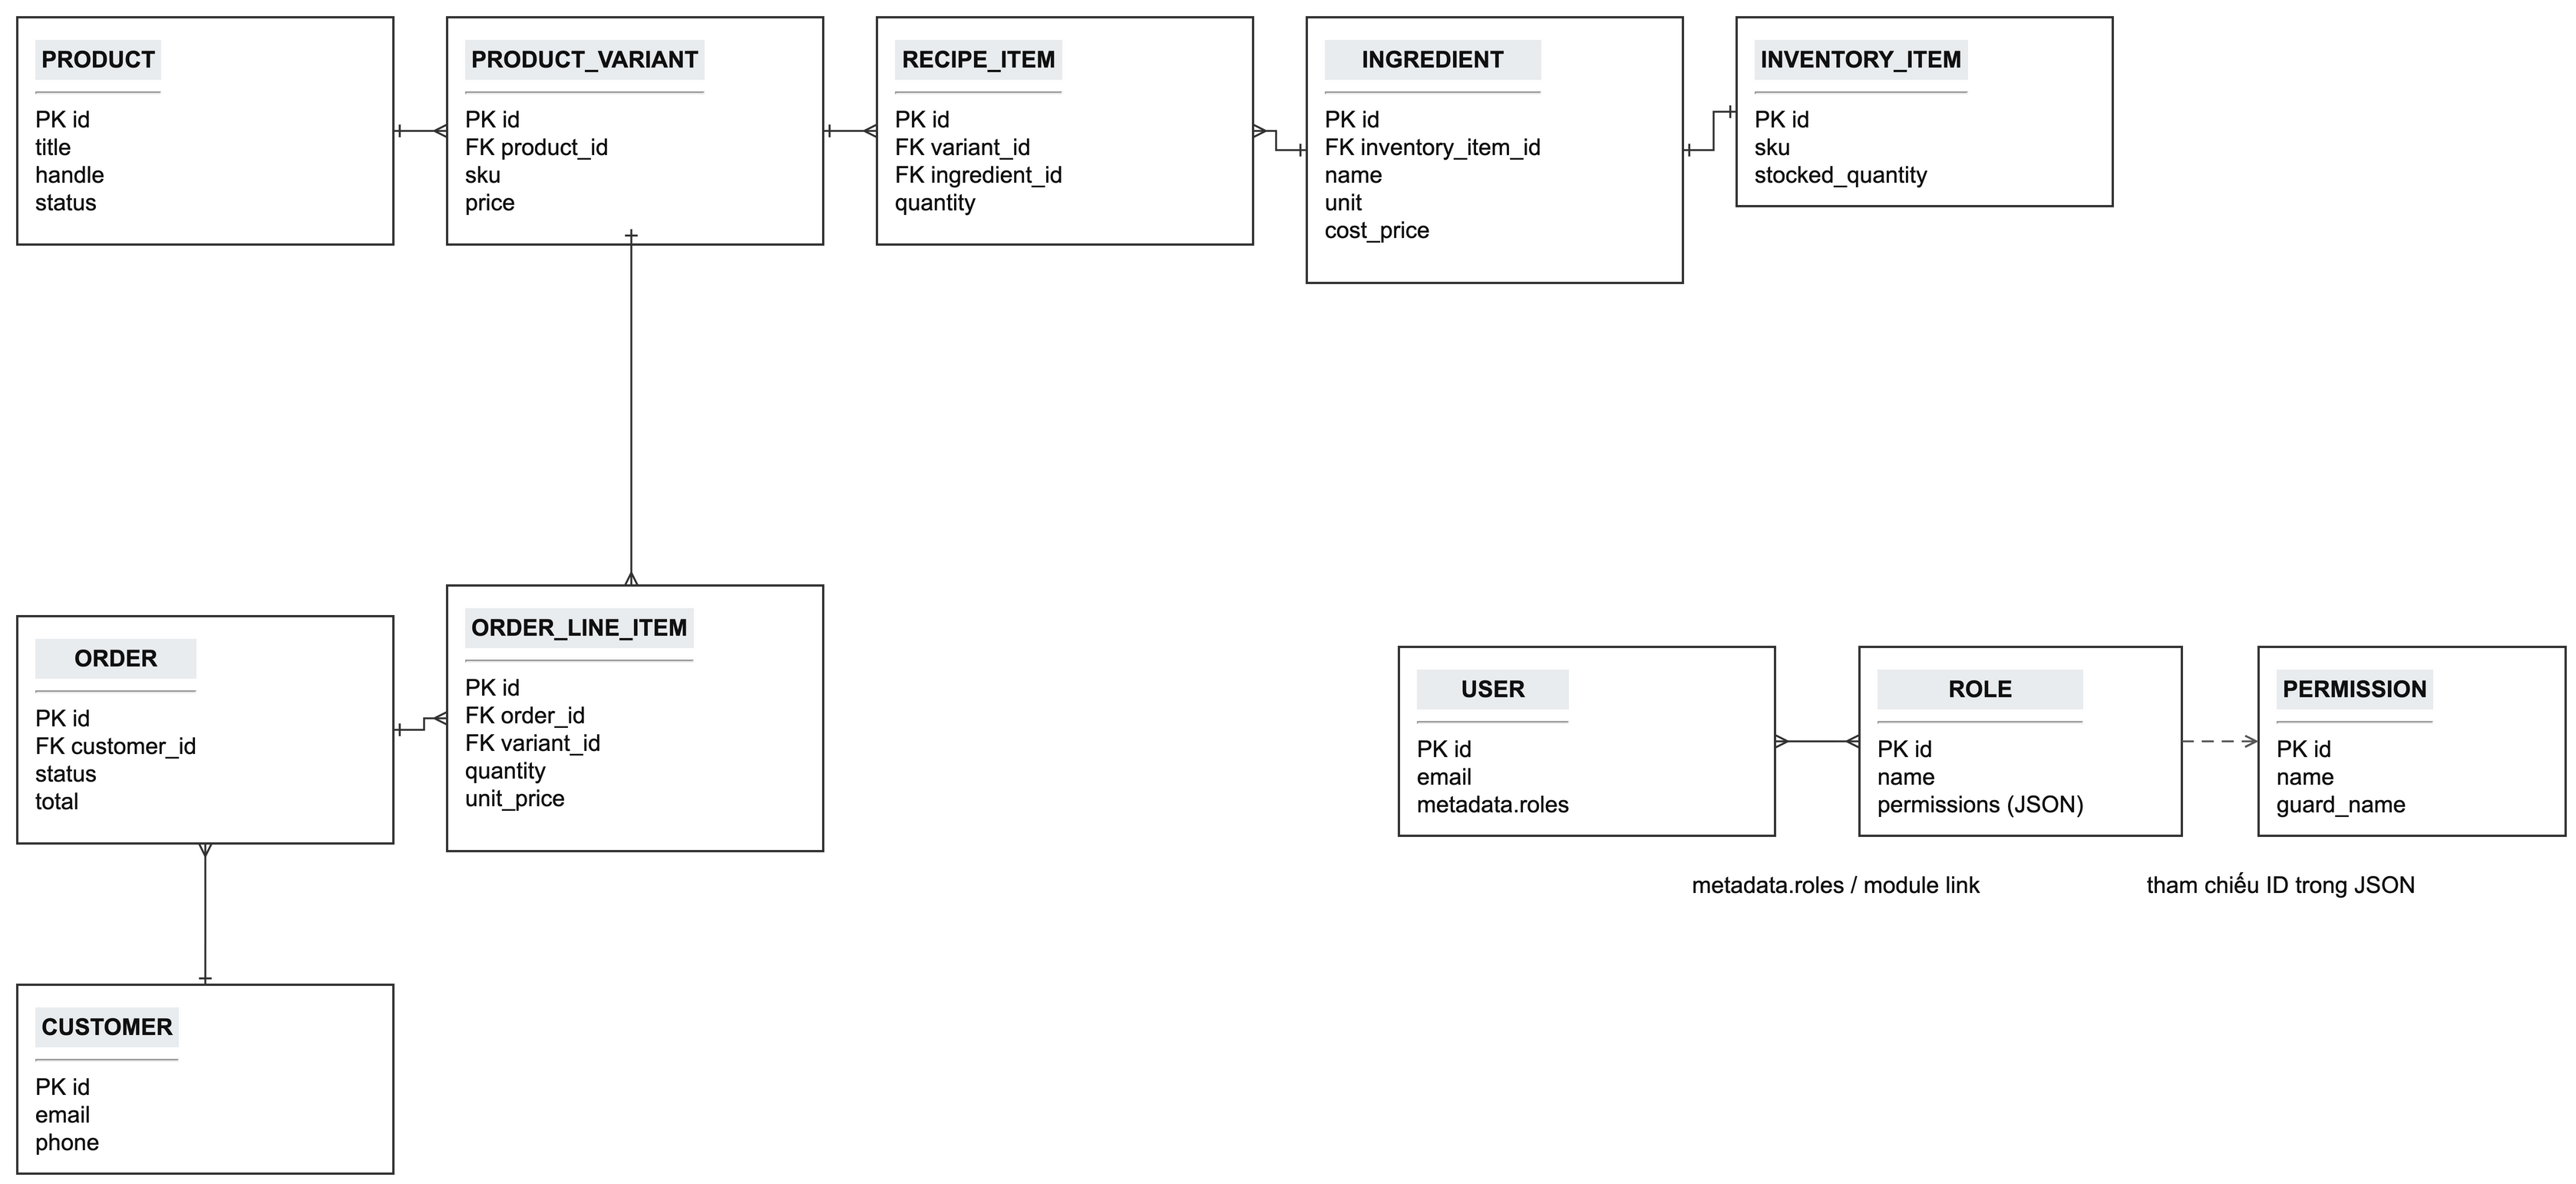
\includegraphics[width=\linewidth,height=0.52\textheight,keepaspectratio]{images/erd.drawio.png}
  \caption{ERD logic của các thực thể nghiệp vụ chính}
  \label{fig:data-links}
\end{figure}
\end{diagramcanvas}

BlogCategory có quan hệ một-nhiều với BlogPost. User liên kết Role; Role tham chiếu Permission. Ingredient liên kết InventoryItem, còn RecipeItem nối biến thể với Ingredient.

\section{Ánh Xạ Mô Hình Miền Sang Lưu Trữ}

ERD chỉ trình bày các bảng quan trọng để giữ khả năng đọc. Trong triển khai thực tế, Medusa tách giá, kho, địa chỉ và liên kết module thành nhiều bảng chuyên biệt. Product--ProductVariant và Order--OrderLineItem là các quan hệ sở hữu; RecipeItem là thực thể kết hợp mang thuộc tính \texttt{quantity}; RBAC đi qua module link hoặc bảng liên kết thay vì làm rò rỉ model của module lõi vào module tùy biến.

Các khóa nghiệp vụ cần ràng buộc duy nhất gồm handle sản phẩm, SKU biến thể, email đăng nhập và tên quyền trong cùng guard. Khóa ngoại hoặc module link thường dùng để lọc cần có index, nhất là các liên kết từ order tới customer và từ recipe item tới variant/ingredient. Truy vấn danh sách cần index kết hợp theo trạng thái và thời gian tạo thay vì tải toàn bộ bản ghi rồi lọc tại ứng dụng.

Lược đồ hiện tại tập trung vào catalog, order, RBAC, site content, ingredient và inventory. Các bảng không còn phục vụ chức năng hiện hành không được đưa vào ERD để sơ đồ gọn và đúng với mã nguồn mới nhất.

\section{Nhất Quán Giao Dịch}

Checkout chạm tới nhiều loại dữ liệu: giá và catalog, số lượng nguyên liệu, promotion, order và event hậu xử lý. PostgreSQL nên bao phủ phần ghi giao dịch cốt lõi; các tác vụ ngoài giao dịch như cập nhật Meilisearch hoặc gửi email nên đi qua event/outbox và có retry. Khóa idempotency phải gắn với kết quả tạo đơn để cùng một request lặp lại trả về cùng order thay vì trừ tồn hai lần. Với tồn kho cạnh tranh, bước giữ hoặc trừ hàng cần khóa/điều kiện cập nhật nguyên tử, không chỉ đọc số lượng rồi ghi lại.

\section{Dữ Liệu Phi Quan Hệ}

\subsection{Redis}

Redis lưu cache có TTL, rate-limit counter và giỏ hàng phiên. Trong development, Redis có thể tắt bằng cấu hình; hệ thống sử dụng implementation giả hoặc localStorage để giảm phụ thuộc. Trong production, Redis cũng có thể làm event bus nhằm xử lý subscriber ngoài tiến trình request.

\subsection{Meilisearch}

Mỗi tài liệu tìm kiếm được suy ra từ Product và các quan hệ liên quan. Các trường được tìm kiếm gồm title, description, slug và tên danh mục; trường lọc gồm trạng thái, category và price range; trường sort gồm thời gian và giá. PostgreSQL vẫn là nguồn dữ liệu chuẩn, còn Meilisearch là bản sao tối ưu truy vấn.

\subsection{MinIO}

MinIO cung cấp API tương thích S3. Cơ sở dữ liệu chỉ lưu object key hoặc URL; dữ liệu nhị phân được lưu trong bucket \texttt{mong-media}. API media quản trị chịu trách nhiệm upload, liệt kê và xóa object.

\section{Toàn Vẹn, Sao Lưu và Bảo Mật Dữ Liệu}

\enlargethispage{2\baselineskip}
\begin{itemize}[leftmargin=2em, itemsep=4pt]
  \item Migration của từng mô-đun phải được áp dụng đồng bộ với phiên bản mã nguồn.
  \item PostgreSQL và bucket MinIO cần được sao lưu; chỉ mục Meilisearch có thể dựng lại từ catalog.
  \item Secret kết nối, khóa Groq, Meilisearch master key và thông tin MinIO không được dùng giá trị mặc định ở production.
  \item API không trả dữ liệu cá nhân cho chatbot; lịch sử đơn được lọc theo customer ID từ token.
  \item Checkout nhiều bước cần workflow có giao dịch và hoàn tác để bảo đảm tính nguyên tử.
\end{itemize}

% ============================================================
%  05_giaodien.tex – Chương 5: Thiết kế giao diện
% ============================================================
\chapter{Thiết Kế Giao Diện}

\section{Định Hướng Thiết Kế}

Frontend sử dụng phong cách ấm, tươi và gần gũi với ngành hàng trái cây. Màu cam được dùng cho hành động chính; ảnh sản phẩm giữ vai trò trung tâm; bố cục card và khoảng trắng giúp người dùng quét nhanh danh sách. Giao diện quản trị ưu tiên mật độ thông tin, bảng dữ liệu và bộ lọc.

Các nguyên tắc chính gồm:

\begin{itemize}[leftmargin=2em, itemsep=4pt]
  \item \textbf{Nhất quán:} dùng chung header, footer, card sản phẩm, trạng thái và hệ thống màu.
  \item \textbf{Responsive:} lưới sản phẩm, form checkout và navigation thay đổi theo chiều rộng màn hình; mobile có bottom navigation.
  \item \textbf{Phản hồi:} các request có loading/error/empty state; thao tác giỏ hàng có toast; nút submit bị khóa trong lúc xử lý.
  \item \textbf{Giảm ma sát mua hàng:} giỏ được lưu lại, checkout chấp nhận khách vãng lai và phí giao hàng hiển thị trước khi đặt đơn.
  \item \textbf{Phân quyền:} menu và route quản trị chỉ hiển thị khi người dùng có quyền tương ứng.
\end{itemize}

\section{Sơ Đồ Điều Hướng Frontend}

Luồng mua hàng chính được tổ chức ngắn gọn theo chuỗi: \textit{Trang chủ/Danh mục/Tìm kiếm} $\rightarrow$ \textit{Chi tiết sản phẩm hoặc hộp tự chọn} $\rightarrow$ \textit{Giỏ hàng} $\rightarrow$ \textit{Checkout} $\rightarrow$ \textit{Xác nhận đơn}. Khách đã đăng nhập có thể đi tiếp tới lịch sử đơn; blog, liên hệ và chính sách là các nhánh nội dung độc lập từ thanh điều hướng chung. Cấu trúc này giữ hành động mua hàng trong tối đa vài bước rõ ràng và vẫn cho phép khám phá nội dung thương hiệu.

\section{Các Màn Hình Khách Hàng}

\begin{longtable}{@{}p{0.25\textwidth} p{0.24\textwidth} p{0.43\textwidth}@{}}
  \toprule
  \textbf{Màn hình} & \textbf{Đường dẫn} & \textbf{Chức năng} \\
  \midrule
  \endhead
  Trang chủ & \texttt{/} & Banner động, nhóm danh mục, sản phẩm nổi bật và nội dung thương hiệu. \\
  Danh sách sản phẩm & \texttt{/products} & Lưới sản phẩm, lọc, sắp xếp và điều hướng tới chi tiết. \\
  Chi tiết sản phẩm & \texttt{/products/:slug} & Ảnh, mô tả, biến thể, giá, số lượng, thành phần và thêm giỏ. \\
  Danh mục & \texttt{/categories/:slug} & Danh sách sản phẩm trong một danh mục động. \\
  Tìm kiếm & \texttt{/search} & Từ khóa, lọc danh mục/mức giá và trạng thái không có kết quả. \\
  Hộp tự chọn & \texttt{/custom-box/:slug} & Tạo cấu hình hộp theo lựa chọn thành phần và ngân sách. \\
  Giỏ hàng & \texttt{/cart} & Chọn dòng hàng, đổi số lượng, xóa và chuyển sang checkout. \\
  Checkout & \texttt{/checkout} & Người nhận, định vị, phí ship, mã khuyến mãi, tóm tắt và đặt đơn. \\
  Tài khoản & \texttt{/account} & Thông tin người dùng và điều hướng tới lịch sử đơn. \\
  Lịch sử đơn & \texttt{/order-history} & Danh sách đơn của khách đang đăng nhập và mã đơn hiển thị. \\
  Blog & \texttt{/blog/:id} & Danh sách và nội dung bài viết theo dữ liệu CMS. \\
  Trang tĩnh & \texttt{/about-us}, \texttt{/contact}, các policy & Giới thiệu, liên hệ, thanh toán, giao hàng và quyền riêng tư. \\
  \bottomrule
\end{longtable}

\section{Ảnh Chụp Giao Diện Từ Phiên Chạy Thử}

Các hình dưới đây được chụp trực tiếp tại \texttt{localhost:5173}. Bộ ảnh được chọn theo hành trình sử dụng thay vì chụp mọi route: sáu màn hình khách hàng bao quát khám phá--cấu hình--tư vấn--checkout và bốn màn hình quản trị bao quát KPI--catalog--đơn hàng--tồn kho. Dữ liệu catalog, giá, ảnh, giỏ hàng và KPI đều đến từ API của dự án, không phải mockup tĩnh.

\begin{figure}[H]
  \centering
  \begin{subfigure}[t]{0.49\textwidth}
    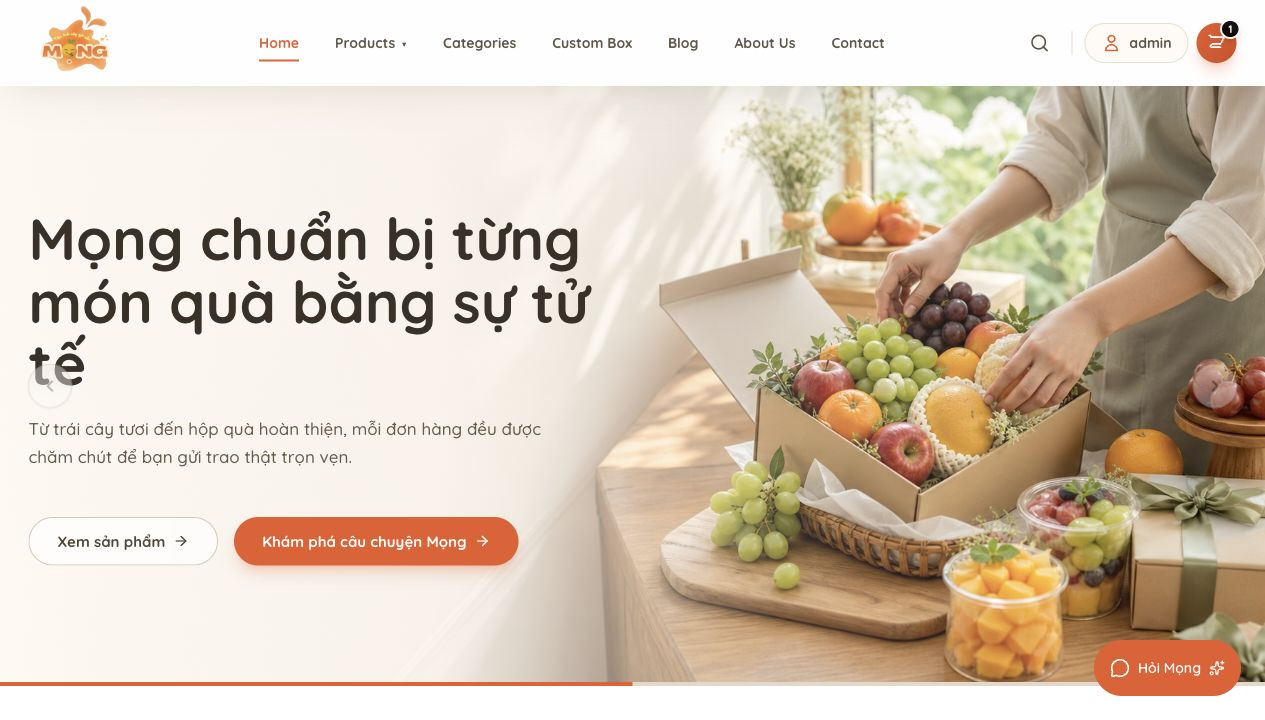
\includegraphics[width=\linewidth]{images/ui-home.png}
    \caption{Trang chủ và nhận diện thương hiệu}
  \end{subfigure}\hfill
  \begin{subfigure}[t]{0.49\textwidth}
    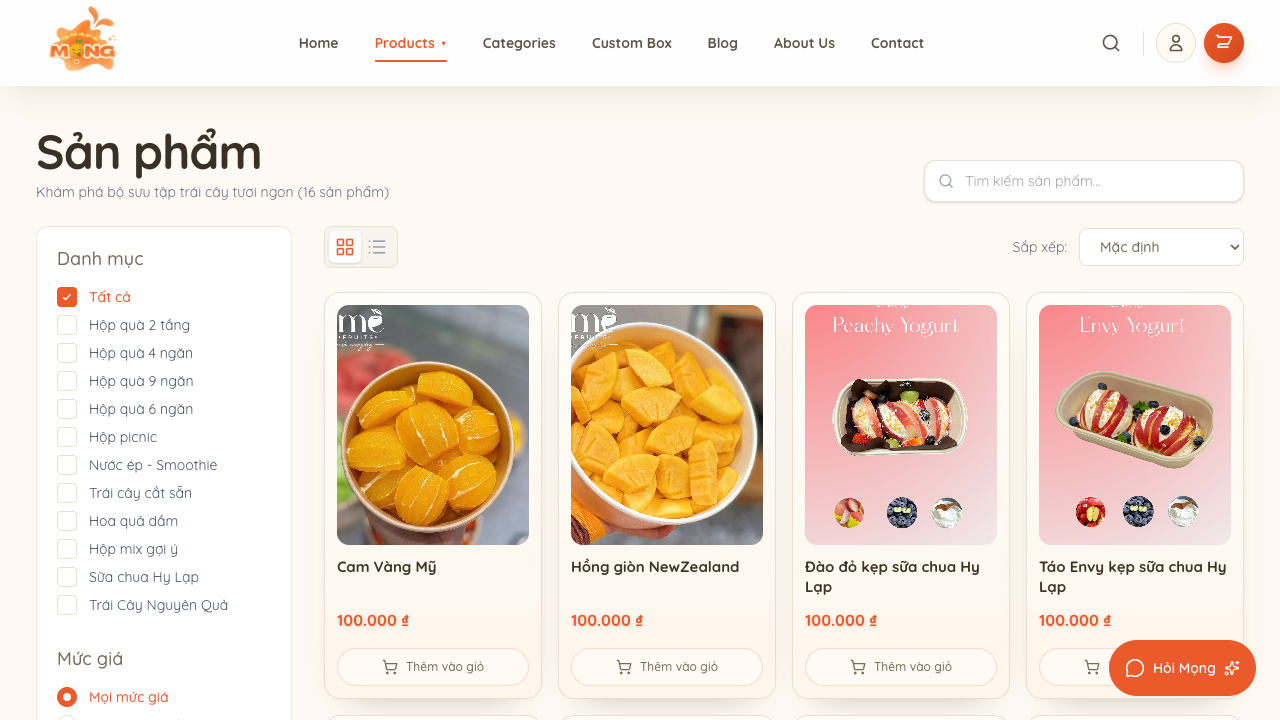
\includegraphics[width=\linewidth]{images/ui-products.png}
    \caption{Catalog và bộ lọc sản phẩm}
  \end{subfigure}
  \caption{Hai điểm vào chính của hành trình khám phá sản phẩm}
  \label{fig:ui-discovery}
\end{figure}

\begin{figure}[H]
  \centering
  \begin{subfigure}[t]{0.49\textwidth}
    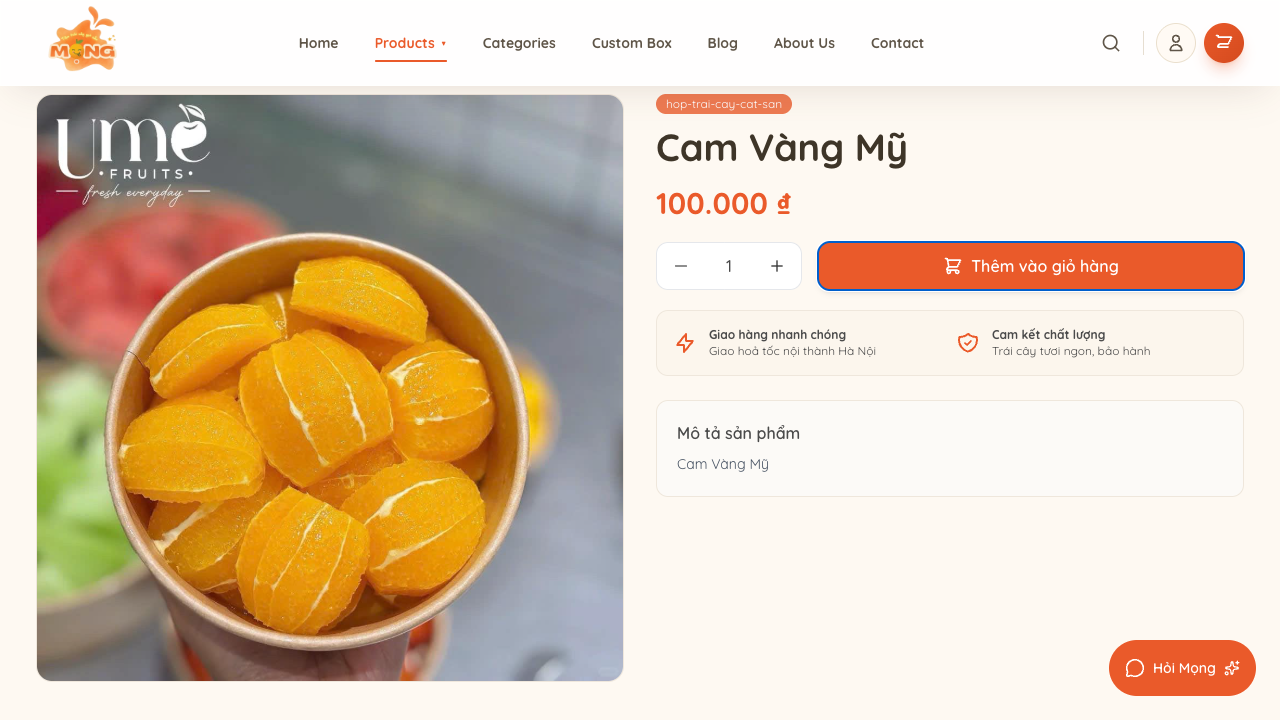
\includegraphics[width=\linewidth]{images/ui-product-detail.png}
    \caption{Chi tiết sản phẩm và biến thể}
  \end{subfigure}\hfill
  \begin{subfigure}[t]{0.49\textwidth}
    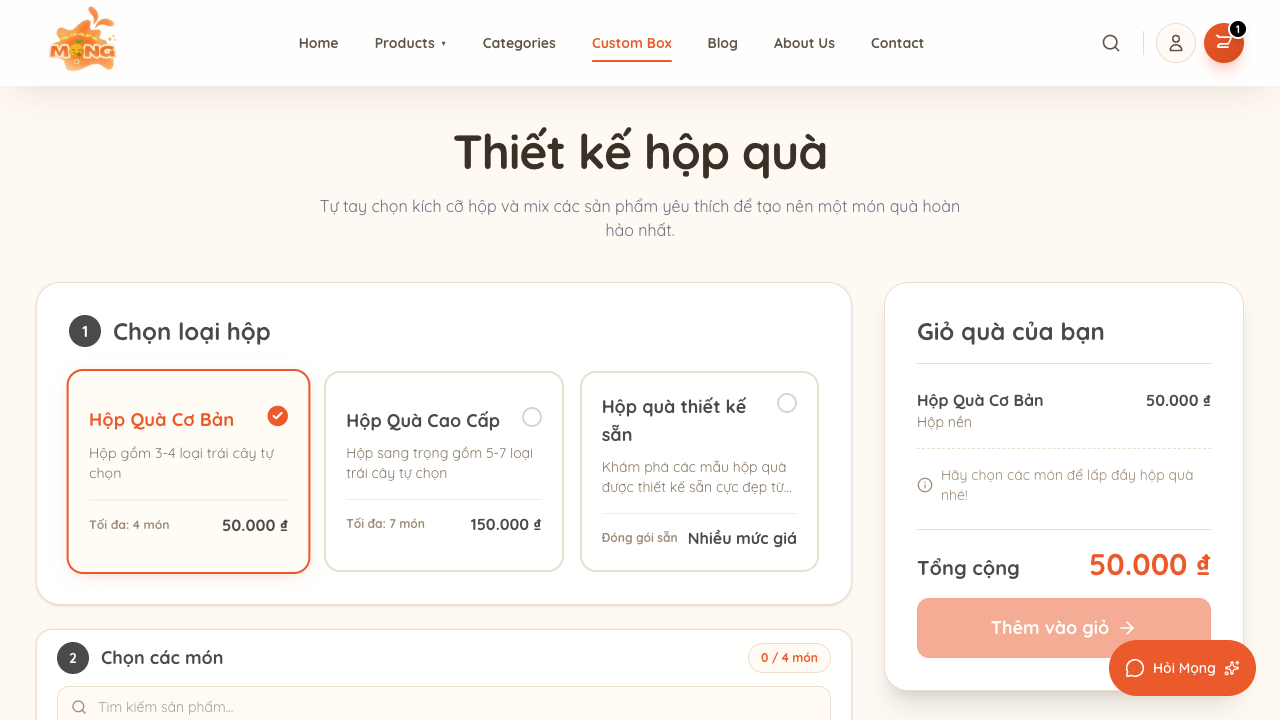
\includegraphics[width=\linewidth]{images/ui-custom-box.png}
    \caption{Tùy chọn thành phần hộp quà}
  \end{subfigure}
  \caption{Hai cách cấu hình sản phẩm trước khi thêm vào giỏ}
  \label{fig:ui-product-config}
\end{figure}

\begin{figure}[H]
  \centering
  \begin{subfigure}[t]{0.49\textwidth}
    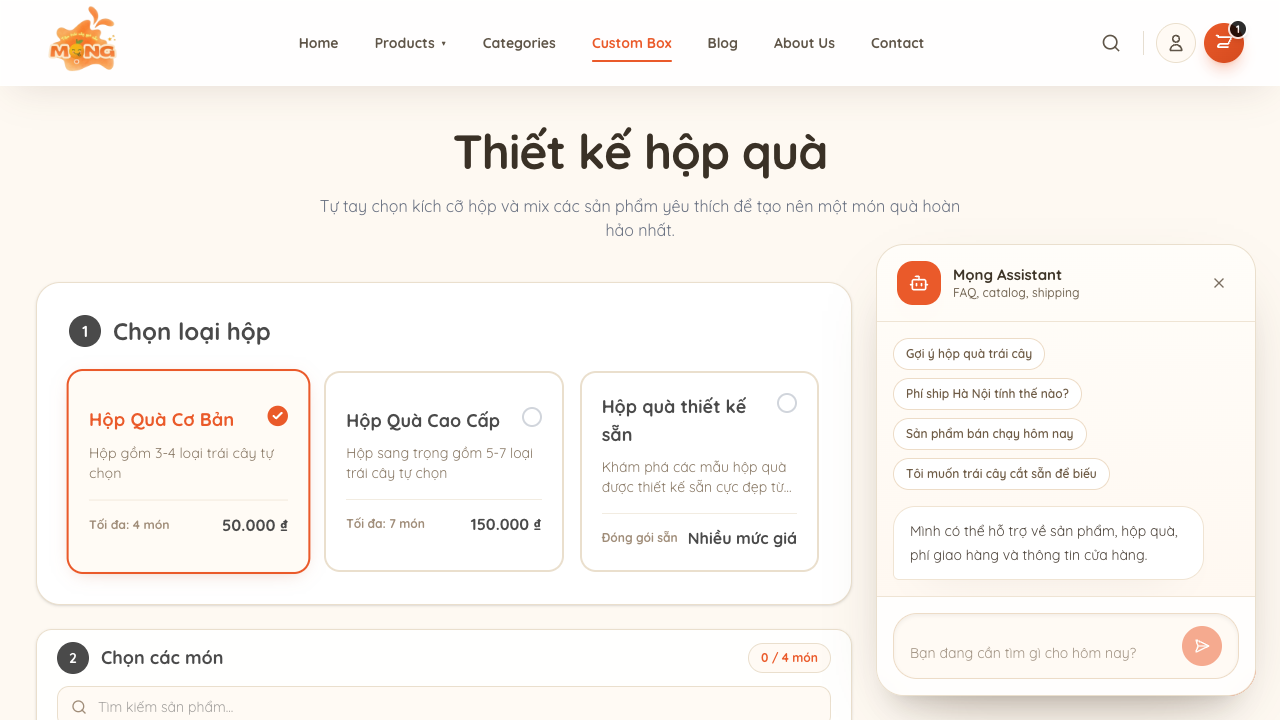
\includegraphics[width=\linewidth]{images/ui-chatbot.png}
    \caption{Chatbot tư vấn trong ngữ cảnh frontend}
  \end{subfigure}\hfill
  \begin{subfigure}[t]{0.49\textwidth}
    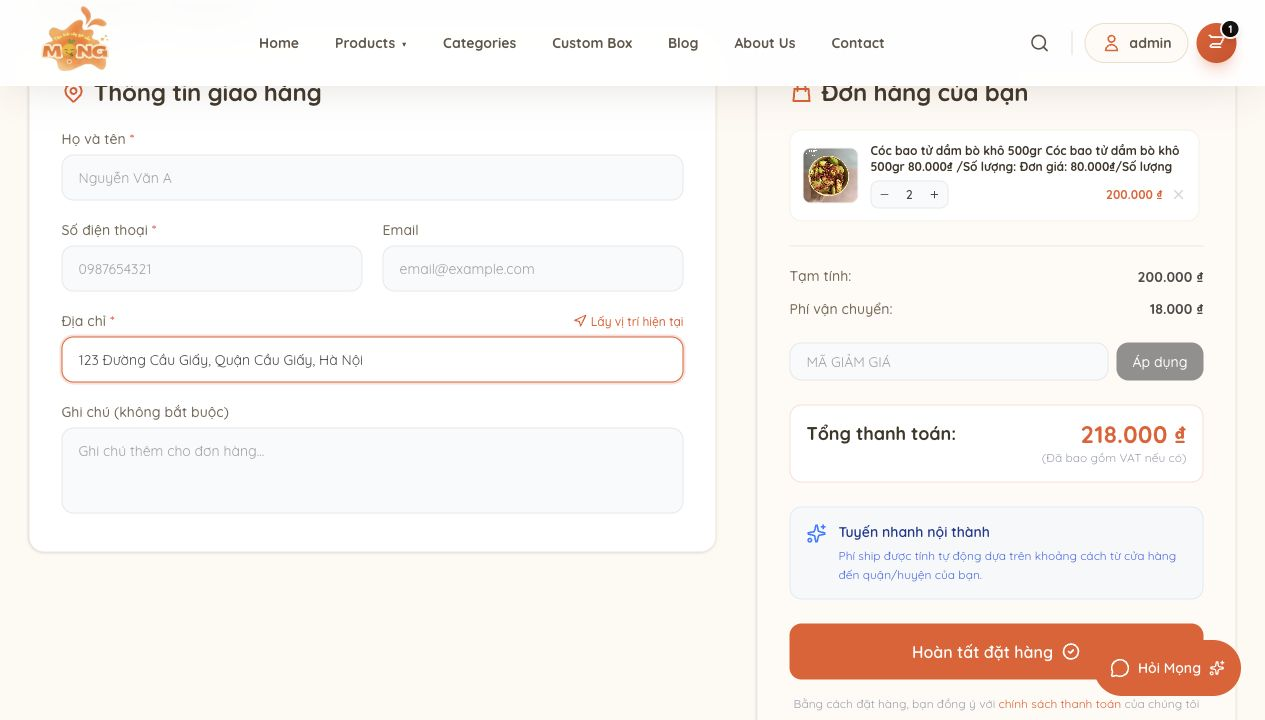
\includegraphics[width=\linewidth]{images/ui-checkout.png}
    \caption{Checkout và tóm tắt tổng đơn}
  \end{subfigure}
  \caption{Hỗ trợ quyết định mua và hoàn tất đơn hàng}
  \label{fig:ui-assist-checkout}
\end{figure}

\subsection{Trang sản phẩm và chi tiết}

Card sản phẩm gom ảnh, tên, giá và hành động mua. Trang chi tiết dùng route động theo slug, nhờ đó không cần tạo file riêng cho từng sản phẩm. Khi sản phẩm có nhiều biến thể, người dùng phải chọn biến thể trước khi thêm vào giỏ. Giao diện review và thao tác gửi điểm đã được loại bỏ; phần dưới trang tập trung vào mô tả, thành phần nguyên liệu và sản phẩm liên quan.

\subsection{Giỏ hàng và checkout}

Giỏ hàng cho phép chọn một phần sản phẩm để checkout. Tại trang checkout, số lượng vẫn có thể chỉnh; hệ thống tính subtotal, giảm giá, phí giao hàng và tổng. Người dùng có thể lấy tọa độ hiện tại để reverse geocode hoặc nhập địa chỉ thủ công. Phí ship được debounce khi địa chỉ thay đổi và có cách tính offline dự phòng cho các quận Hà Nội.

\subsection{Chatbot}

ChatbotWidget xuất hiện trên frontend dưới dạng nút nổi. Câu trả lời hỗ trợ Markdown và có thể kèm card gợi ý sản phẩm. UI cần phân biệt trạng thái đang gửi, lỗi giới hạn tần suất và phản hồi fallback để khách hiểu mức độ chắc chắn của thông tin.

Qua phiên chạy thử, bố cục khách hàng có thứ bậc thị giác rõ: hành động chính dùng màu cam, nội dung bán hàng dùng card và ảnh lớn, chatbot nổi ở góc nhưng không che nút checkout. Điểm nên cải thiện là thống nhất chiều cao ảnh sản phẩm, tăng tương phản một số chữ phụ và hiển thị rõ hơn nguồn tính phí giao hàng trước khi người dùng xác nhận.

\section{Khu Vực Quản Trị}

Quản trị được đặt dưới namespace \texttt{/admin}. \texttt{AdminLayout} cung cấp sidebar, header và vùng nội dung; \texttt{ProtectedRoute} yêu cầu đăng nhập; \texttt{RequirePermission} chặn các màn hình cần quyền cụ thể.

\begin{longtable}{@{}p{0.27\textwidth} p{0.26\textwidth} p{0.39\textwidth}@{}}
  \toprule
  \textbf{Nhóm quản trị} & \textbf{Route tiêu biểu} & \textbf{Nghiệp vụ} \\
  \midrule
  \endhead
  Dashboard & \texttt{/admin}, \texttt{/admin/finance} & KPI tổng quan, doanh thu, chi phí và lợi nhuận. \\
  Catalog & \texttt{/admin/products}, \texttt{/admin/categories} & CRUD sản phẩm, biến thể, ảnh và danh mục. \\
  Kho và nguyên liệu & \texttt{/admin/inventory}, \texttt{/admin/ingredients} & Mức tồn, giá vốn, loại nguyên liệu và công thức. \\
  Bán hàng & \texttt{/admin/orders}, \texttt{/admin/promotions} & Theo dõi đơn, trạng thái và điều kiện khuyến mãi. \\
  Khách hàng & \texttt{/admin/customers} & Hồ sơ khách hàng và lịch sử mua hàng. \\
  Nội dung & \texttt{/admin/banners}, \texttt{/admin/blog}, \texttt{/admin/media} & Banner, bài viết, danh mục blog và thư viện ảnh. \\
  Cấu hình & \texttt{/admin/settings/*}, \texttt{/admin/content/*} & Giao hàng, website, chính sách và FAQ chatbot. \\
  Vận hành hệ thống & \texttt{/admin/search}, \texttt{/admin/chatbot} & Trạng thái chỉ mục và câu hỏi chatbot chưa xử lý. \\
  Phân quyền & \texttt{/admin/users}, \texttt{/admin/roles} & Người dùng nội bộ, role và permission. \\
  \bottomrule
\end{longtable}

Các trang danh sách dùng chung \texttt{AdminListFilters} để tìm kiếm và lọc. Form tạo/sửa được tách thành route riêng. Trạng thái admin được chuẩn hóa bằng các component loading, error và empty để tránh mỗi trang tự định nghĩa cách hiển thị khác nhau.

\begin{figure}[H]
  \centering
  \begin{subfigure}[t]{0.49\textwidth}
    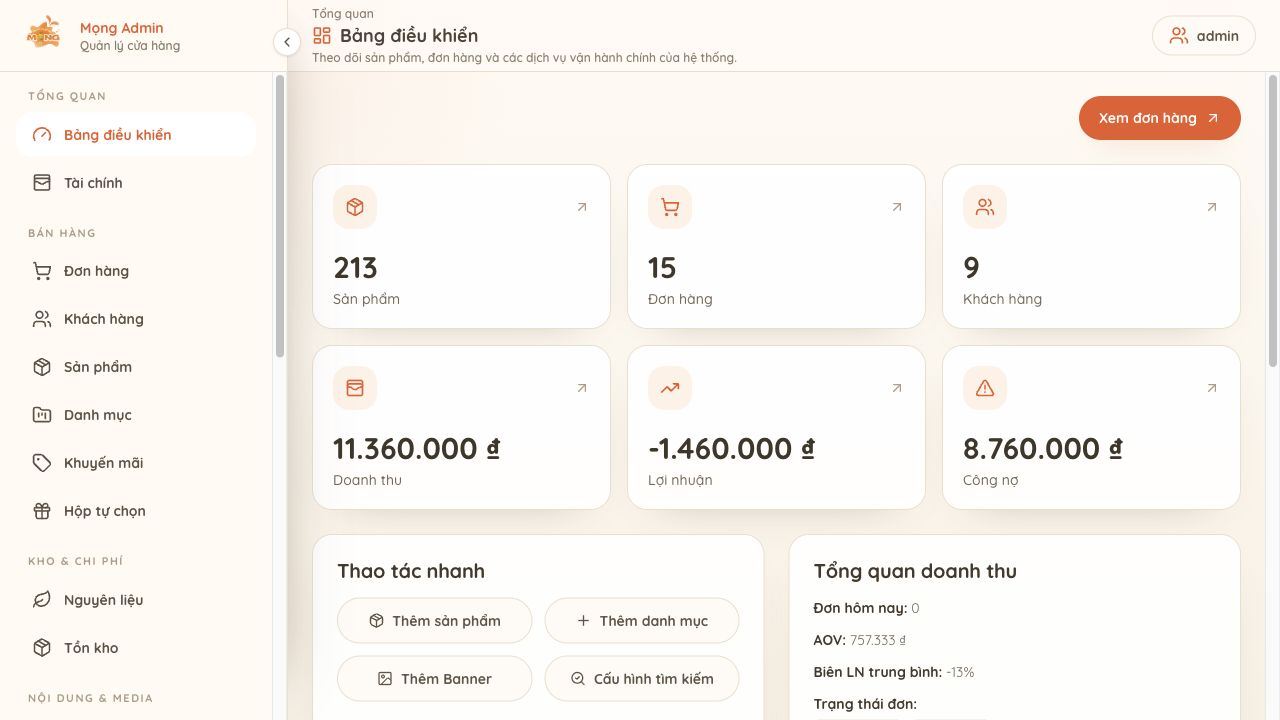
\includegraphics[width=\linewidth]{images/ui-admin-dashboard.png}
    \caption{Dashboard và KPI vận hành}
  \end{subfigure}\hfill
  \begin{subfigure}[t]{0.49\textwidth}
    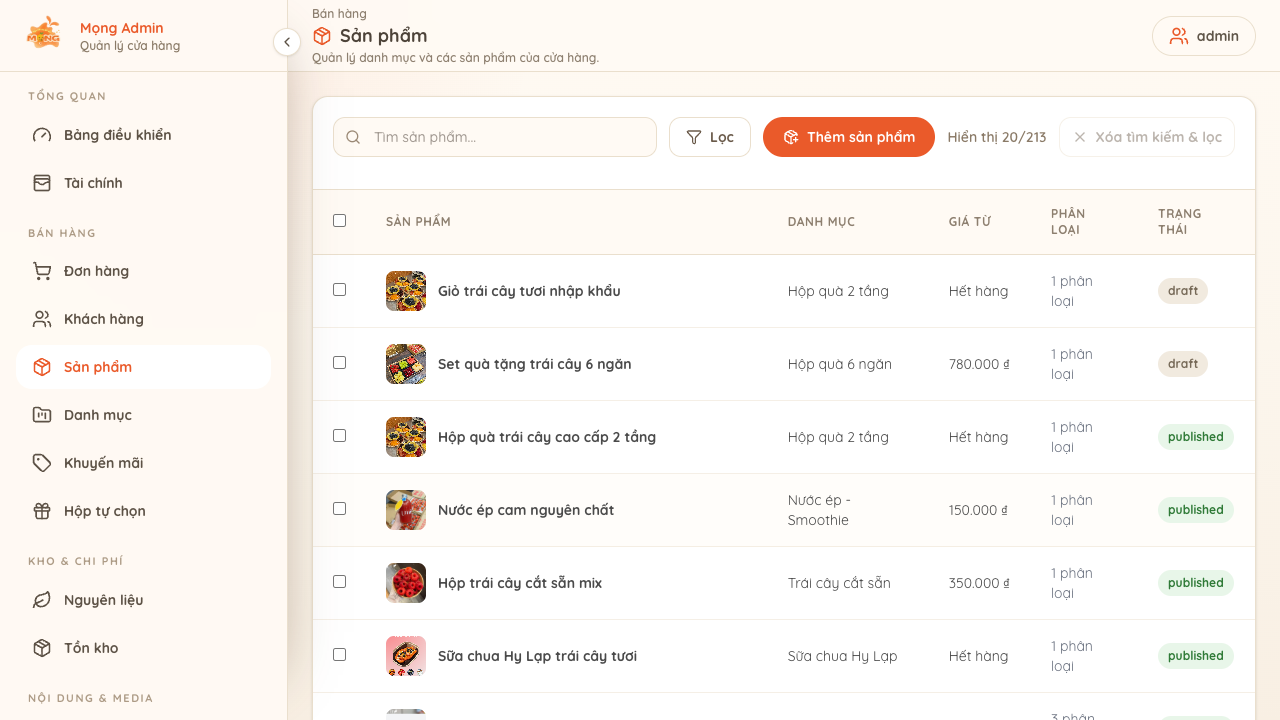
\includegraphics[width=\linewidth]{images/ui-admin-products.png}
    \caption{Danh sách sản phẩm quản trị}
  \end{subfigure}
  \caption{Tổng quan vận hành và quản trị catalog}
  \label{fig:ui-admin-overview}
\end{figure}

\begin{figure}[H]
  \centering
  \begin{subfigure}[t]{0.49\textwidth}
    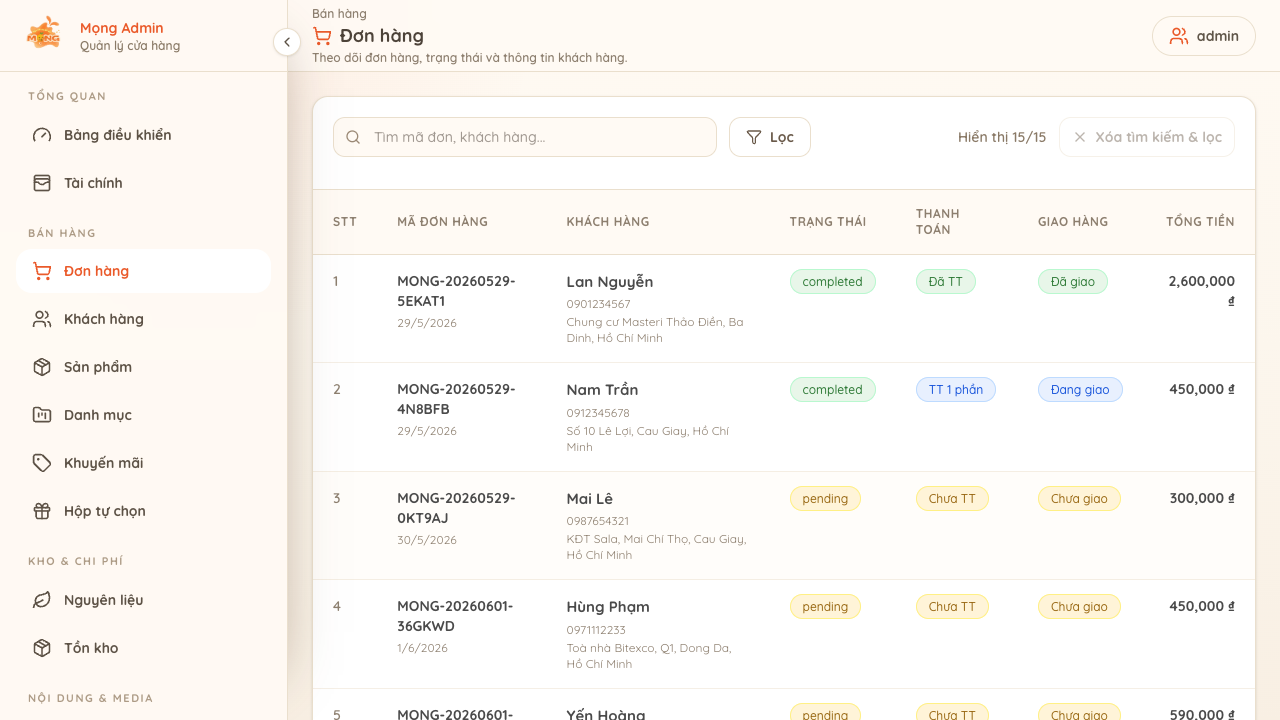
\includegraphics[width=\linewidth]{images/ui-admin-orders.png}
    \caption{Theo dõi đơn hàng và trạng thái}
  \end{subfigure}\hfill
  \begin{subfigure}[t]{0.49\textwidth}
    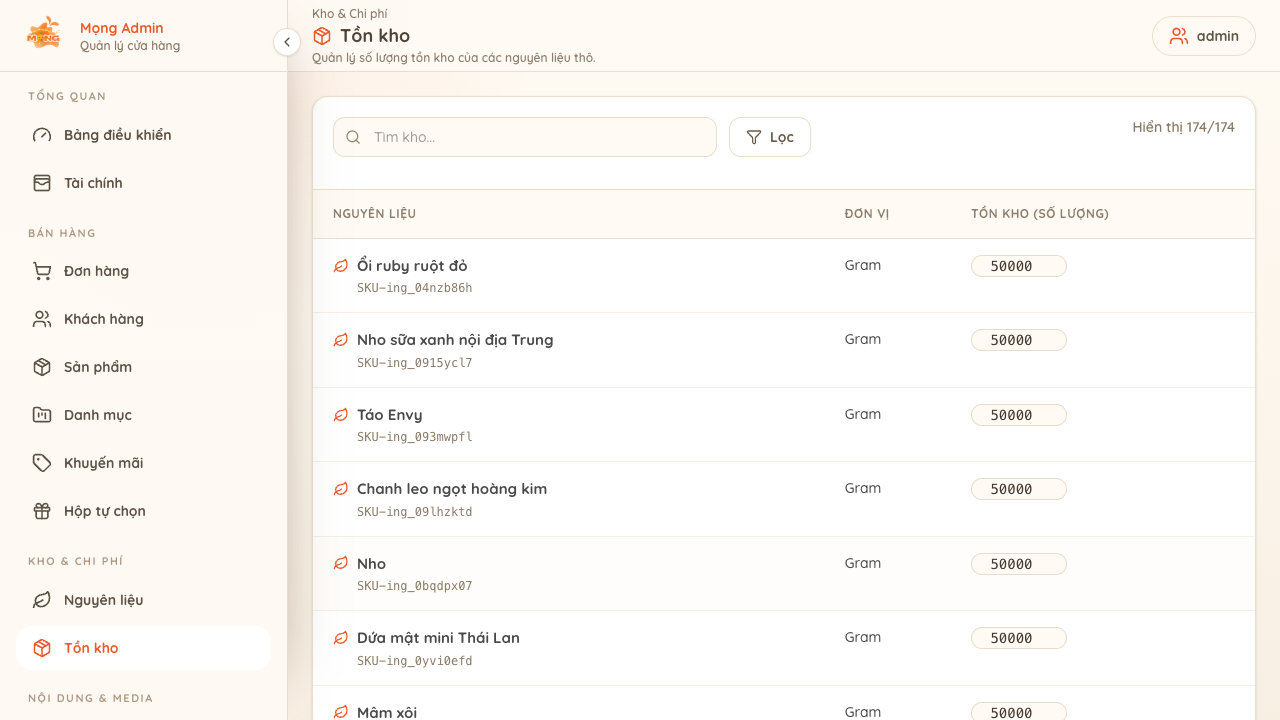
\includegraphics[width=\linewidth]{images/ui-admin-inventory.png}
    \caption{Mức tồn kho theo mặt hàng}
  \end{subfigure}
  \caption{Hai màn hình tác nghiệp bán hàng và kho}
  \label{fig:ui-admin-operations}
\end{figure}

Các bảng quản trị giữ bộ lọc và hành động ở vùng đầu trang, giúp nhân viên chuyển nhanh từ quan sát sang xử lý. Dashboard phù hợp để nhận biết xu hướng; trang đơn hàng cung cấp dữ liệu tác nghiệp; trang tồn kho hỗ trợ quyết định nhập hoặc điều chỉnh hàng. Cần tiếp tục chuẩn hóa tên trạng thái tiếng Việt, định dạng tiền và mật độ cột giữa các bảng để giảm thời gian làm quen.

\section{Khả Năng Tiếp Cận và Responsive}

Một số nền tảng tốt đã có như lazy loading route, bottom navigation trên mobile và nhãn trạng thái rõ ràng. Tuy nhiên, cần tiếp tục rà soát khả năng dùng bàn phím, focus khi mở modal, vùng chạm tối thiểu 44 px và thông báo động cho trình đọc màn hình. Đặc biệt, số lượng giỏ nên dùng \texttt{aria-live="polite"}; ảnh dưới màn hình đầu nên đặt \texttt{loading="lazy"}; trang sản phẩm nên bổ sung JSON-LD và metadata SEO.

\section{Đánh Giá Tính Nhất Quán}

Frontend và admin hiện cùng nằm trong một ứng dụng React nhưng phục vụ hai phong cách sử dụng khác nhau. Cách tổ chức này thuận tiện khi phát triển nhanh, song bundle và design system có thể trở nên lớn. Trong giai đoạn tiếp theo có thể tách admin thành workspace riêng hoặc chuyển các phần quản trị phù hợp sang Medusa Admin extensions, đồng thời chuẩn hóa màu, typography, component bảng và form dùng chung.

% ============================================================
%  06_tongket.tex – Chương 6: Tổng kết
% ============================================================
\chapter{Tổng Kết}

\section{Kết Quả Triển Khai}

Dự án đã xây dựng được một nền tảng thương mại điện tử cho Mọng Fruitboxz với hai khu vực sử dụng chính: giao diện mua sắm cho khách hàng và giao diện quản trị cho cửa hàng. Ở phía khách hàng, hệ thống hỗ trợ duyệt catalog, xem chi tiết sản phẩm, tìm kiếm, chọn biến thể, quản lý giỏ hàng, áp dụng khuyến mãi, tự động báo phí giao hàng và đặt đơn. Khách hàng đã đăng nhập có thêm khả năng quản lý tài khoản và theo dõi lịch sử mua hàng.

Ở phía vận hành, hệ thống cung cấp các chức năng quản lý sản phẩm, danh mục, đơn hàng, khách hàng, khuyến mãi, tồn kho, nguyên liệu, banner, blog, media, FAQ, cấu hình website và người dùng nội bộ. Một đặc thù nghiệp vụ được thể hiện trong đề tài là mô hình tồn kho theo công thức nguyên liệu: mỗi biến thể sản phẩm có thể được cấu thành từ nhiều nguyên liệu khác nhau, nhờ đó quá trình đặt hàng phản ánh gần hơn nghiệp vụ bán trái cây cắt sẵn và hộp quà.

Về mặt tổ chức hệ thống, dự án đã tách rõ giao diện, backend, dữ liệu và các dịch vụ hỗ trợ. Backend Medusa được mở rộng bằng các mô-đun riêng cho nội dung, phân quyền, nguyên liệu, yêu cầu mua số lượng lớn và giao hàng. Frontend sử dụng React để xây dựng trải nghiệm mua hàng và khu vực quản trị trong cùng một mã nguồn, đồng thời kết nối với các dịch vụ tìm kiếm, lưu trữ ảnh và chatbot tư vấn.

\section{Đối Chiếu Kết Quả Theo Nhóm Chức Năng}

\begin{longtable}{@{}L{0.27\textwidth} L{0.25\textwidth} L{0.40\textwidth}@{}}
  \toprule
  \textbf{Nhóm chức năng} & \textbf{Hiện trạng triển khai} & \textbf{Minh chứng và giới hạn} \\
  \midrule
  \endhead
  Catalog và tìm kiếm & Đã triển khai luồng chính & Sản phẩm, biến thể, danh mục, ảnh và bộ lọc đã có trên giao diện; backend có cơ chế trả kết quả dự phòng khi dịch vụ tìm kiếm không khả dụng. \\
  Giỏ hàng và đặt hàng & Đã triển khai đặt đơn; thanh toán còn ở mức ghi nhận & Người dùng có thể thêm sản phẩm, chỉnh số lượng, nhập thông tin nhận hàng, áp dụng khuyến mãi và tạo đơn. Phí giao hàng được tính lại ở backend; thanh toán trực tuyến chưa được tích hợp. \\
  Giao hàng theo khu vực & Đã có cấu hình và báo phí tự động & Hệ thống có gợi ý địa chỉ, định vị, báo phí theo quận/khoảng cách và lưu thông tin giao hàng trong đơn; lịch giao và đối tác vận chuyển chưa được mô hình hóa sâu. \\
  Quản trị vận hành & Đã có các màn hình nghiệp vụ chính & Khu vực quản trị bao phủ catalog, đơn hàng, khách hàng, khuyến mãi, tồn kho, nội dung và phân quyền; thao tác hàng loạt và cách gọi trạng thái vẫn cần làm chặt hơn. \\
  Nội dung và chăm sóc khách hàng & Đã có CMS và kênh tư vấn cơ bản & Banner, blog, FAQ, liên hệ và chatbot đã được kết nối với dữ liệu dự án; chất lượng tư vấn phụ thuộc vào việc bổ sung FAQ và dữ liệu sản phẩm khi vận hành. \\
  Tồn kho theo nguyên liệu & Đã có mô hình BOM & Công thức BOM liên kết sản phẩm bán ra với lượng nguyên liệu thực tế; nếu dùng cho cửa hàng thật, cần xử lý kỹ hơn phần cạnh tranh tồn kho và nhập/xuất kho. \\
  Báo cáo vận hành & Có dashboard tổng quan & Dashboard đã hiển thị một số chỉ số doanh thu, chi phí, lợi nhuận và công nợ; phân tích theo thời gian, nhóm sản phẩm và hiệu quả khuyến mãi là hướng mở rộng. \\
  \bottomrule
\end{longtable}

\section{Những Điểm Cần Hoàn Thiện}

\begin{itemize}[leftmargin=2em, itemsep=5pt]
  \item \textbf{Thanh toán trực tuyến:} hiện đơn hàng chủ yếu dừng ở ghi nhận đơn và hướng dẫn chuyển khoản. Nếu triển khai thực tế, cần kết nối cổng thanh toán phù hợp và có cơ chế xác nhận trạng thái thanh toán.
  \item \textbf{Thông báo sau đặt hàng:} email xác nhận và thông báo cho nhân viên cửa hàng cần được kết nối với nhà cung cấp gửi thư hoặc kênh nhắn tin thật.
  \item \textbf{Quy trình giao vận:} trạng thái giao hàng đã được mô hình hóa ở mức cơ bản; có thể bổ sung lịch giao, khu vực phục vụ, người phụ trách và ghi chú xử lý đơn.
  \item \textbf{Báo cáo kinh doanh:} dashboard hiện cho cái nhìn tổng quan; phần phân tích doanh thu, chi phí, lợi nhuận, tồn kho và hiệu quả khuyến mãi theo thời gian còn có thể trình bày sâu hơn.
  \item \textbf{Trải nghiệm quản trị:} một số màn hình quản trị có nhiều chức năng; nên thống nhất lại cách lọc, tìm kiếm, phân trang và thao tác nhanh để nhân viên sử dụng thuận tiện hơn.
  \item \textbf{Nội dung tư vấn:} chatbot đã hỗ trợ hỏi đáp cơ bản; chất lượng câu trả lời sẽ tốt hơn khi FAQ, dữ liệu sản phẩm và kịch bản tư vấn được bổ sung thường xuyên từ quá trình vận hành thực tế.
\end{itemize}

\section{Hướng Phát Triển}

\begin{itemize}[leftmargin=2em, itemsep=5pt]
  \item Tích hợp thanh toán trực tuyến, đối soát giao dịch và hiển thị trạng thái thanh toán rõ ràng cho khách hàng.
  \item Hoàn thiện thông báo đơn hàng qua email, SMS hoặc kênh nội bộ để nhân viên xử lý đơn nhanh hơn.
  \item Mở rộng cấu hình giao hàng theo khung giờ, khu vực phục vụ, phí theo thời điểm và lựa chọn đơn vị vận chuyển.
  \item Phát triển báo cáo quản trị theo ngày, tuần, tháng, nhóm sản phẩm, khách hàng và hiệu quả chương trình khuyến mãi.
  \item Cải thiện chatbot theo hướng ghi nhận câu hỏi phổ biến, gợi ý sản phẩm chính xác hơn và hỗ trợ nhân viên bổ sung FAQ từ trang quản trị.
  \item Cải thiện phiên bản mobile và nội dung SEO để website dùng tốt hơn trong bối cảnh bán hàng thật.
\end{itemize}

\section{Kiến Thức và Kinh Nghiệm Thu Được}

Quá trình thực hiện giúp sinh viên củng cố cách xây dựng một hệ thống thương mại điện tử theo kiến trúc headless commerce, cách tách giao diện khách hàng khỏi backend, cách tổ chức dữ liệu sản phẩm--đơn hàng--tồn kho và cách mở rộng Medusa bằng các mô-đun riêng. Đề tài cũng là dịp luyện kỹ năng đọc mã nguồn lớn, đối chiếu giữa giao diện và nghiệp vụ, vẽ sơ đồ phân tích--thiết kế, cũng như trình bày kết quả thành một báo cáo có cấu trúc.

Một kinh nghiệm quan trọng là chức năng bán hàng không chỉ nằm ở trang sản phẩm hay nút đặt mua. Để tạo được một luồng mua hàng hoàn chỉnh, hệ thống phải phối hợp nhiều phần: dữ liệu sản phẩm, giá bán, tồn kho, phí giao hàng, khuyến mãi, tài khoản khách hàng, trạng thái đơn và công cụ cho nhân viên vận hành.

\section{Kết Luận}

Mọng Fruitboxz đã triển khai được các thành phần chính của một website bán hàng cho cả khách hàng và cửa hàng. Hệ thống thể hiện được đặc thù của sản phẩm trái cây qua biến thể, hộp quà, giao hàng theo khu vực, chatbot tư vấn và tồn kho theo nguyên liệu. Dù vẫn còn các phần cần hoàn thiện như thanh toán trực tuyến, thông báo sau đặt hàng và báo cáo chuyên sâu, phiên bản hiện tại vẫn đủ để làm nền cho các bước phát triển tiếp theo của hệ thống.

\section{Tài Liệu Tham Khảo}

\begin{enumerate}[leftmargin=2em, itemsep=4pt]
  \item Medusa Documentation. \url{https://docs.medusajs.com/}
  \item React Documentation. \url{https://react.dev/}
  \item Vite Documentation. \url{https://vite.dev/guide/}
  \item Tailwind CSS Documentation. \url{https://tailwindcss.com/docs}
  \item PostgreSQL 15 Documentation. \url{https://www.postgresql.org/docs/15/}
  \item Redis Documentation. \url{https://redis.io/docs/latest/}
  \item Meilisearch Documentation. \url{https://www.meilisearch.com/docs/}
  \item MinIO Documentation. \url{https://min.io/docs/minio/}
  \item Docker Compose Documentation. \url{https://docs.docker.com/compose/}
  \item Groq API Documentation. \url{https://console.groq.com/docs/}
  \item Mã nguồn Mọng Fruitboxz. \url{https://github.com/pathust/mong.fruitboxz}
\end{enumerate}


\end{document}
